\chapter{مروری بر ادبیات و کار‌های انجام شده}
\clearpage
\section{پروپوزال}
هدف های پيش بيني شده و روش ها و ضرورت انجام طرح :
1-	بررسی ترابرد بار و اسپین در بورفین:
بوروفن و گرافن به دلیل داشتن صفحات ضخیم اتمی منفرد شباهت زیادی دارند و دارای ساختار محکم زیادی هستند که انعطاف پذیری فوق العاده ای را به نمایش می گذارد. با این حال ، آنها تمایز قابل توجهی در ساختارهای شبکه خود دارند. بوروفن یک آلوتروپ کریستالی از بور است که به عنوان یک ساختار عمده دارای طبیعت غیر فلزی است. بوروفن ماده ای بسیار ناهمسانگرد است که رفتارهای نیمه رسانا و فلزی را نشان می دهد. اخیراً ، نانوساختار نویدبخش دو بعدی از نظر تئوری پیش بینی شده است و اثرات شکست تقارن سوراخ ذرات توسط هدایت نوری گزارش شده است [46]. علاوه بر این ، اخیراً خواص \lr{ab initio 8-Pmmn borophene} مورد مطالعه قرار گرفته است [47] و \lr{Li} و همکاران. [48] طیف انرژی \lr{8-Pmmn borophene}را بدست آورد و نشان داد که ماده ایده آل برای تجزیه و تحلیل تونل سازی کلاین در حضور ناهمسانگردی است. بعلاوه ، مشابه اثرات میدان مغناطیسی گرافن نیز در این ماده پرداخته شده است [49] اما هنوز هم برای تعیین کاربردهای عملی آن به کارهای زیادی نیاز دارد.

در [50] نشان داده شده است که اولا طیف انرژی الکترونیکی ناهمسانگرد است ثانیا طیف ناهمسانگرد با پتانسیل مثلث گسترش یافته است .
در [50] نشان داده شده‌ است که  ترکیب‌های گوناگون از صفحه‌های بورن وجود دارد و همچنین اثرا بررسی نشده بسیاری باقی‌مانده است که می‌توان آنها را محاسبه کرد.
\begin{figure*}[!ht]
    \centering
    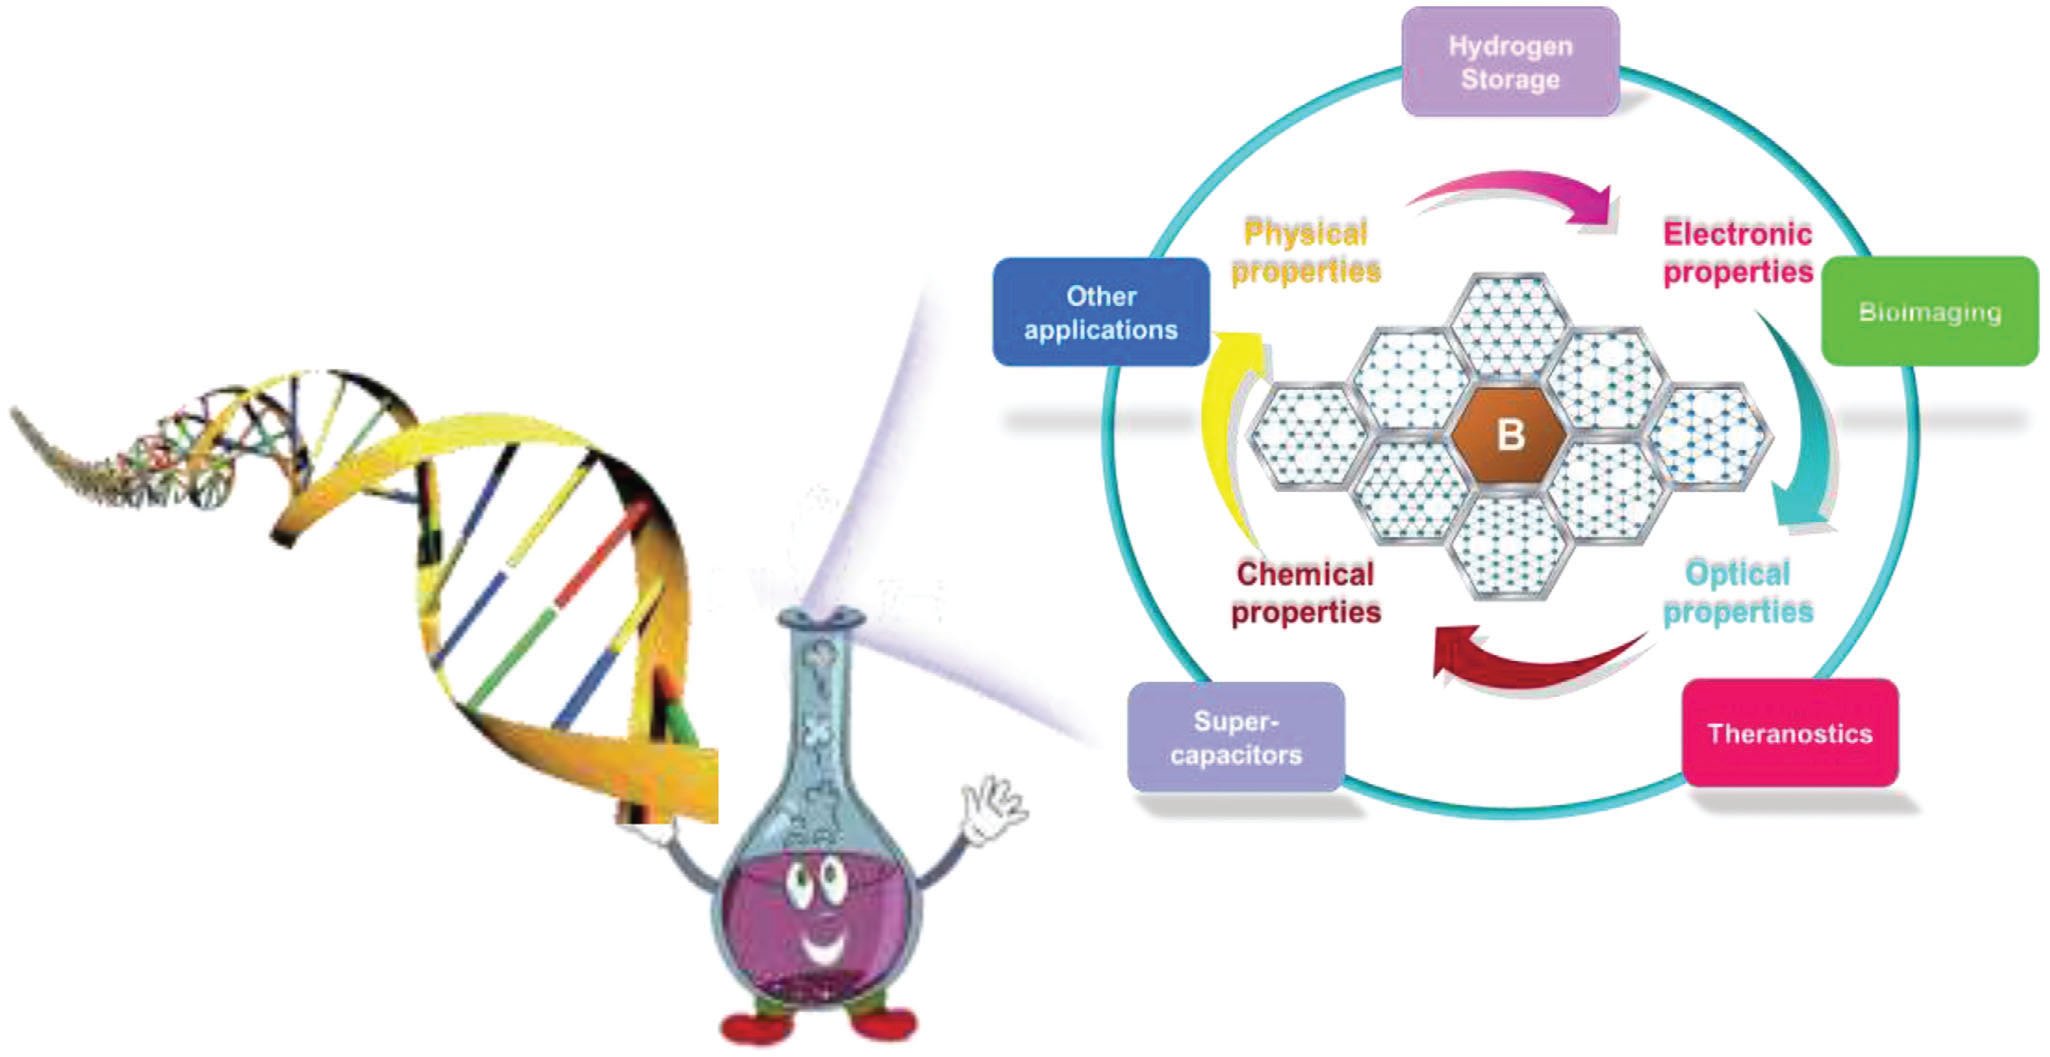
\includegraphics[width=\linewidth]{borophenedev.png}
    \caption{تصویری از توسعه منحصر به فرد بوروفن. نظریه های بوروفن فراوان است. اطلاعات کلیدی موثر بر خواص و سنتز بوروفن از طریق پیش‌بینی نظری، مشابه سنتز پروتئین مبتنی بر ژن، به دست آمده است تا به طور کلی سنتز بوروفن را هدایت کند.}
    \label{fig:borophenedev}
\end{figure*}
\section{مقدمه:}
نانومواد دو بعدی به دلیل ویژگی های منحصر به فرد و فوق العاده شان توجه زیادی را از جامعه علمی به خود جلب کرده اند.\cite{huangGraphenebasedComposites2012, huangGrapheneBasedMaterialsSynthesis2011}بر خلاف مواد توده ای\LTRfootnote{\lr{Bulk}}، ورقه های نانویی فوق نازک دو بعدی که اکثر اتم هایشان در معرض سطح قرار دارند، دارای سطح ویژه بزرگتر، فعالیت شیمیایی و فیزیکی بالاتر و اثرات محصوریت کوانتومی\LTRfootnote{Quantum confinement} هستند که به آنها ویژگی های خاص فوتونی، الکترونیکی، کاتالیزوری و مغناطیسی می بخشد و پتانسیل کاربردی بالایی در مواد زیست سازگار، حامل های دارو، بیوسنسورها، وسایل الکترونیکی و غیره دارند.\cite{lu2DTransitionMetalDichalcogenideNanosheetBasedComposites2016, chhowallaChemistryTwodimensionalLayered2013, sunElectronicStructuresSiC2008} در سال 2004 ظهور گرافن باعث تحول بزرگی در حوزه مواد شد و کاربردهای مواد دو بعدی را در زمینه های مختلف به طور چشمگیری بهبود بخشید. \cite{novoselovElectricFieldEffect2004, geimRiseGraphene2007} با این حال، شکاف باند صفر گرافن بسیاری از کاربردهای آن را در قطعات الکترونیکی، تصویربرداری زیستی و فتودینامیک تراپی محدود می کند. در سال های اخیر، محققان به دنبال یافتن مواد دو بعدی با ساختار لانه زنبوری مانند گرافن یا ورقه های نانویی دو بعدی تک عنصری هستند که در گروه همانند یا مجاور عنصر کربن قرار دارند، به امید توسعه مواد مشابه گرافن با خواص عالی. خوشبختانه ظهور مواد دارای ساختار مشابه گرافن مانند سولفیدهای فلزات واسطه \lr{(\ch{TMDs})}\cite{dingDefectEngineeredBioactive2019, liRatiometricImmunoassaysBuilt2019}، نیترید بور مربعی \lr{(\ch{h}-\ch{BN})}\cite{deanBoronNitrideSubstrates2010}،و نیترید بور گرافیتی \lr{(\ch{g}-\ch{C3N4})}\cite{caoPolymericPhotocatalystsBased2015}و همچنین مواد دو بعدی تک عنصری مانند بوروفن\cite{fengExperimentalRealizationTwodimensional2016}،سیلسین\cite{fengEvidenceSiliceneHoneycomb2012,chenEvidenceDiracFermions2012,duTuningBandGap2014}، استانن\cite{gouStraininducedBandEngineering2017, zhuEpitaxialGrowthTwodimensional2015}،و ژرمانن \cite{niTunableBandgapSilicene2012} نه تنها می توانند کمبود شکاف باند صفر گرافن را جبران کنند، بلکه دارای خواص ویژه دیگری نیز هستند که انتظار می رود عملکردها و کاربردهای جدیدی را به ارمغان بیاورند. در مقایسه با سایر مواد دو بعدی، نانوموادهای تک عنصری دارای سه مزیت منحصر به فرد هستند: 1) سازگاری بیشتر با فناوری نیمه هادی موجود. به عنوان مثال، عناصر سیلیسیم و ژرمانیم عناصر اصلی ساخت مواد نیمه هادی سنتی هستند. 2) به دلیل تشکیل شده از یک عنصر، سنتز با کیفیت بالا نسبتا ساده است. 3) تجزیه و متابولیزه شدن توسط سیستم های بیولوژیکی آسان تر است. فسفر سیاه یکی از نانوموادهای دو بعدی تک عنصری با سازگاری زیستی خوب است. این ماده می تواند در بدن به فسفات تجزیه شود و در حفظ بسیاری از فعالیت های فیزیولوژیکی مهم به عنوان ماده اولیه برای \lr{ATP} و \lr{DNA} شرکت کند.\cite{shaoBiodegradableBlackPhosphorusbased2016,taoBlackPhosphorusNanosheets2017}علاوه بر این، سطح ویژه بسیار بالا و سطوح مختلف پاسخ به \lr{pH}، نور، الکتریسیته و غیره، باعث می شود نانوموادهای دو بعدی تک عنصری به گزینه های برتر برای وسایل الکترونیکی، انتقال دارو، درمان نوری، تصویربرداری زیستی و سایر زمینه ها تبدیل شوند. \cite{liEngineeredFunctionalized2D2020,shiPHSensitiveNanoscaleMaterials2020}

همانطور که بوروفن یکی از مواد نانویی تک عنصری دوبعدی به حساب می‌آید، شباهت زیادی به گرافن و فسفر سیاه دارد. نه تنها سطح ویژه‌ای بالا و ظرفیت بارگذاری دارو بالایی دارد (بوروفن: 114\% \cite{jiNovelTopDownSynthesis2018}، فسفر سیاه: 108\% \cite{taoBlackPhosphorusNanosheets2017}، گرافن اکسید: 200\% \cite{zhangFunctionalGrapheneOxide2010}، سایر نانومواد: \lr{10-30\%}، بلکه در شرایط اسیدی، نوری و حرارتی قادر به رهاسازی دارو به صورت هوشمندانه نیز هست. بوروفن یکی از مرموزترین نانوموادهای تک عنصری دوبعدی است که منحصر به فردترین ویژگی‌اش چندشکلی\LTRfootnote{Polymorphism} بودن (چند ساختار متفاوت داشتن) آن است. بوروفن‌هایی که با روش‌های مختلف و تحت شرایط گوناگون ساخته می‌شوند، ساختارهای متفاوتی دارند و این دگرشکل‌ها\LTRfootnote{Allotropes} ویژگی‌های گوناگونی هم از خود نشان می‌دهند. برای مثال، پیش‌بینی می‌شود بوروفن فاز \lr{Pmmn} با مخروط‌های دیراک و ویژگی‌های الکتریکی جدید، ماده‌ی جذاب\LTRfootnote{Intriguing} دیراک باشد \cite{zhouSemimetallicTwoDimensionalBoron2014}. خواص فاز $\beta_{12}$ بوروفن و فاز $\alpha$ بوروفن هم تفاوت دارند؛ اولی ناهمسانگرد و دومی همسانگرد است \cite{zhouSuperiorLatticeThermal2017, xiaoLatticeThermalConductivity2017}. این به این معنی است که می‌توانیم با کنترل و تنظیم شرایط ساخت، بوروفن‌هایی را سنتز کنیم که نیازهای کاربردی ما را برآورده کنند. امروزه هنوز گزارش‌های کمی در مورد بوروفن وجود دارد و این ویژگی‌های شگفت‌انگیز مشاهده شده، تنها بخش کوچکی از این کوه یخی هستند؛ هنوز جزئیات بسیاری برای کشف توسط محققان باقی مانده است.

بور، تنها عنصر نیمه‌رسانا در گروه \lr{IIIA} و پنجمین عنصر در جدول تناوبی عناصر، هم‌جوار کربن و دارای اوربیتال‌های ظرفیتی مشابه آن است. \cite{forteInitioPredictionBoron2010}این شباهت‌ها نشان می‌دهد که بوروفن، فلز دوبعدی سبک، ممکن است ویژگی‌های جالب مشابه گرافن داشته باشد. \cite{huangTwoDimensionalBoronPolymorphs2017, liuIntermixingPeriodicSelfassembly2018} ساختار الکترونی خاص، مکانیزم پیوند پیچیده و هم‌بستگی نزدیک با عناصر کربن نشان می‌دهد که بوروفن احتمالا خواص عالی مشابه گرافن خواهد داشت و حتی می‌تواند از آن فراتر رفته و به ابرماده جدیدی تبدیل شود. در واقع، محاسبات نظری حاکی از آن است که بوروفن دارای ساختارهای دگرشکلی کم‌بعدی زیاد و خواص جالبی است. \cite{liuBorophenegrapheneHeterostructures2019} بوستانی و همکاران \cite{boustaniSYSTEMATICLSDINVESTIGATION1994} پیش‌بینی کردند که خوشه‌های بور ممکن است ساختاری شبه صفحه‌ای\LTRfootnote{quasi-planar} تشکیل دهند که نشان می‌دهد بوروفن دوبعدی را می‌توان به‌صورت تجربی تهیه کرد.به‌علت مکانیزم‌های پیوند پیچیده و ساختار غیرلایه‌ای بور توده‌ای، سنتز تجربی بوروفن تا سال 2015 به دست نیامد، زمانی که گروه‌های تحقیقاتی \lr{Guisinger} \cite{mannixSynthesisBorophenesAnisotropic2015} و \lr{Wu} \cite{fengExperimentalRealizationTwodimensional2016} به‌طور جداگانه بر روی \lr{Ag(111)} به سنتز آن دست یافتند. برخلاف اکثر مواد سنتی که با آزمایش‌های تجربی مستقیم طراحی می‌شوند، طراحی بوروفن با نظریه‌هایی آغاز شد که ویژگی‌های بالقوه و روش‌های احتمالی تهیه آن را پیش‌بینی می‌کردند و به‌طور موفقیت‌آمیزی فرآیند تهیه آزمایشگاهی و کاربردهای بعدی بوروفن را هدایت کردند (طرح‌واره 1). توسعه بوروفن بدون شک نمونه موفقی از پروژه ژنوم مواد \lr{(MGI)} است. همانطور که انسان‌ها ژن‌هایی دارند که ویژگی‌های آن‌ها را تعیین می‌کند، مواد نیز دارای «ژن‌های» کلیدی هستند که خواص آن‌ها را مشخص می‌کنند. \lr{MGI} پیش‌نهاد می‌کند قبل از کشف مواد ناشناخته، رابطه بین ترکیب، ساختار و خواص مواد از طریق تحقیقات نظری روشن شود تا کارایی سنتز مواد، هزینه تحقیقات مواد و موفقیت طراحی مواد افزایش یابد. ظهور و تکامل بوروفن الگویی برجسته برای سنتز مواد جدید ارائه می‌دهد.
\begin{figure*}
    \centering
    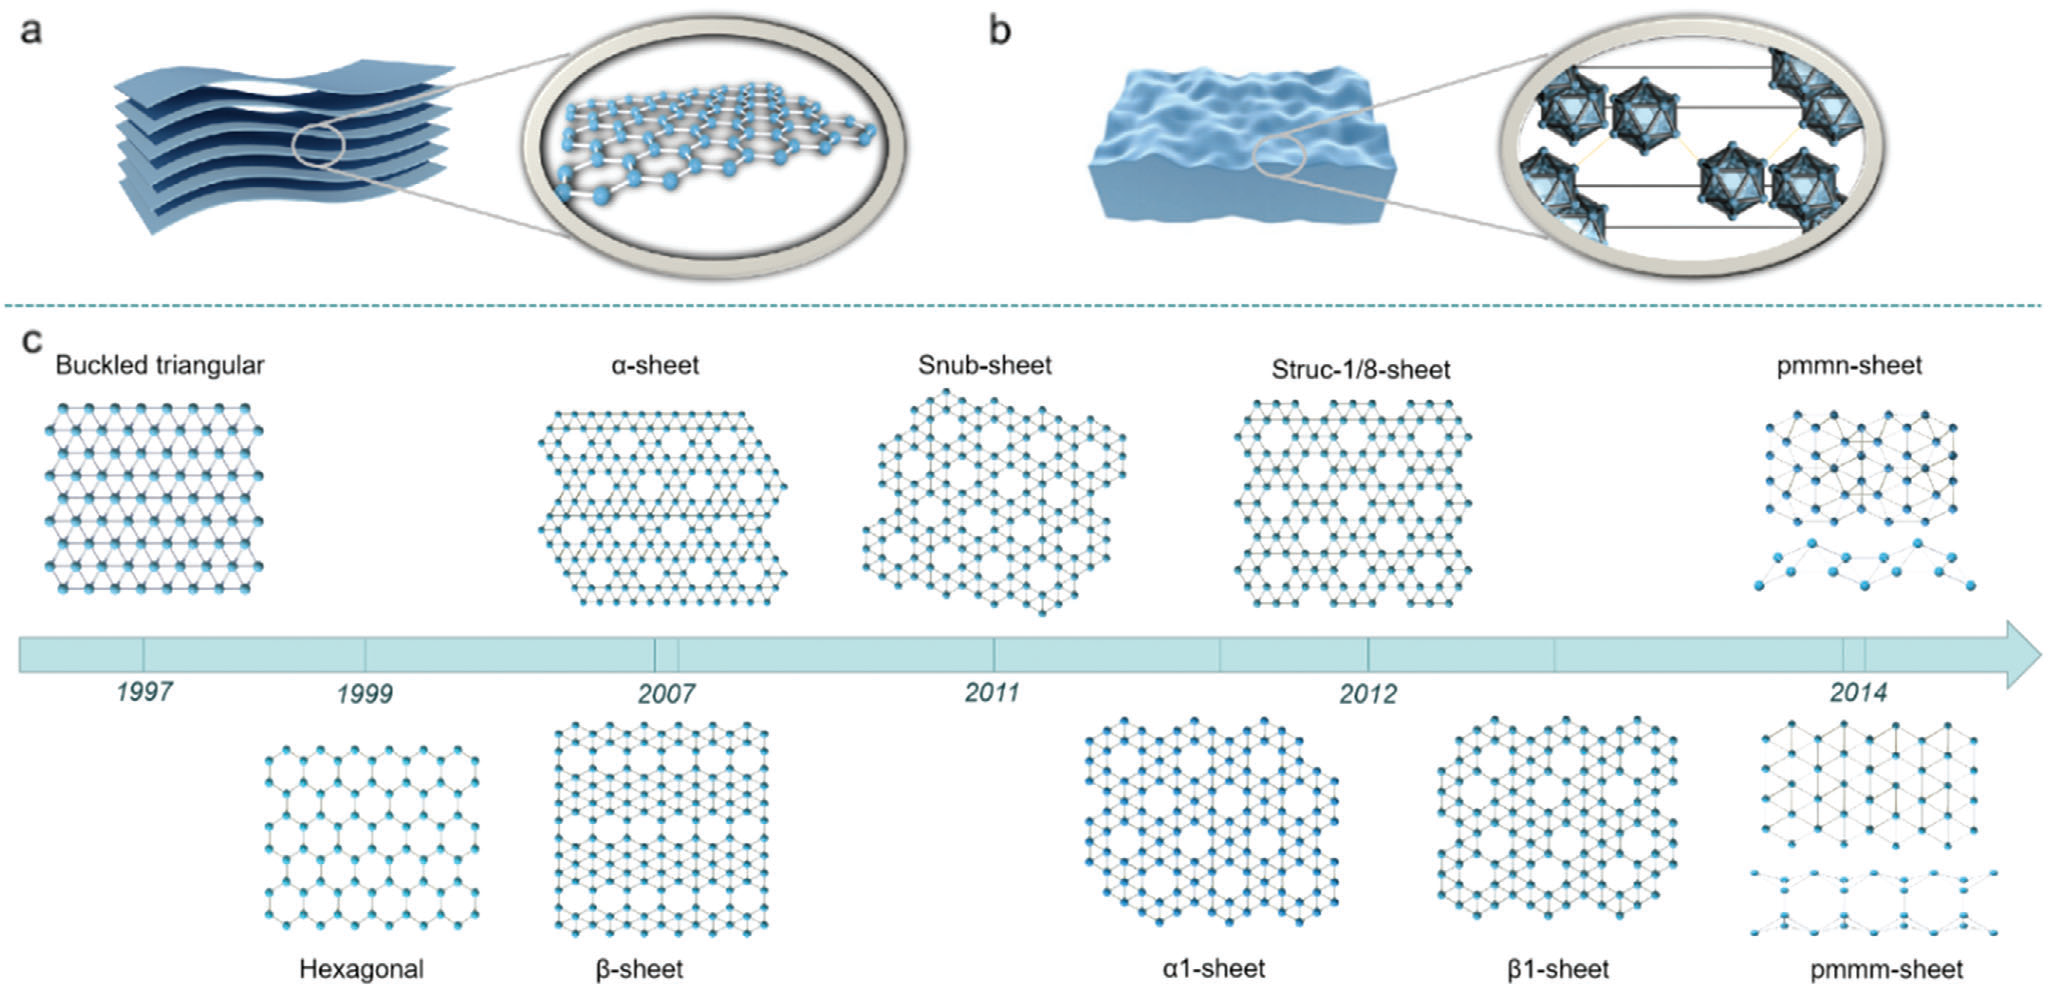
\includegraphics[width=\textwidth]{theory-borophene.png}
    \caption{این شکل باید بازطرحی شود}
    \label{theoryborophene}
\end{figure*}
\section{بررسی تئوری ساختار بور دوبعدی}
به دلیل کمبود الکترون در لایه بیرونی، اتم‌های بور به راحتی می‌توانند پیوندهای شیمیایی تشکیل دهند؛ بنابراین، بور از نظر شیمیایی فعال بوده و ترکیباتی با ساختارهای کریستالی متنوع ایجاد می‌کند. ساختار اصلی کریستالی بور توده (شکل\lr{\ref{theoryborophene}.b}) \LTRfootnote{Icosahedron}بر اساس یک ایکوزاهدرون \ch{12B} به عنوان واحد ساختاری پایه استوار است، و انواع مختلف کریستال‌های بور از طریق اتصالات و روش‌های پیوند مختلف روی ایکوزاهدرون \ch{12B} شکل می‌گیرند. \cite{albertBoronElementaryChallenge2009} بنابراین، توده بور برخلاف گرافن (شکل\lr{\ref{theoryborophene}.a}) یک ساختار لایه‌ای ندارد که باعث پیچیده و دشوار شدن تهیه بوروفن می‌شود.

در سال 2006، \lr{Kunstmann} , \lr{Quandt} \cite{kunstmannBroadBoronSheets2006} برای اولین بار ساختار پایه ورق‌های بور دوبعدی را پیش‌بینی کردند و راز بوروفن را آشکار ساختند. در سال 2014، وانگ و همکاران \cite{zhaiObservationAllboronFullerene2014} برای اولین بار نشان دادند که \ch{36B} یک خوشه بوروفن شبه مسطح بسیار پایدار با ساختار توخالی شش ضلعی است و تأیید کردند که خوشه‌های بوروفن تک اتمی با حفره‌های شش ضلعی امکان‌پذیر هستند. همچنین برای اولین بار مفهوم بوروفن را ارائه دادند. در سال‌های اخیر، تحقیقات تئوری بوروفن به نتایج مثمری رسیده است، اما روش‌های سنتز و کاربردهای بور همچنان اندک هستند.

اولین سنتز بوروفن در آزمایشگاه در سال 2015 به دست آمد. بوروفن دارای انواع ساختارها است که بر اساس الگوهای ترکیب طبقه‌بندی می‌شوند: الف) صفحه شش ضلعی کج‌ و معوج \lr{\ch{(DH)}}، ب) صفحه مثلثی خمیده \lr{\ch{(BT)}}، و ج) صفحه مثلثی-شش ضلعی ترکیبی \lr{\ch{(MTH)}}، یا بر اساس عدد هماهنگی (\lr{CN}): نوع $\alpha$ (\lr{CN = 5، 6})، نوع $\beta$ (\lr{CN = 4، 5، 6})، نوع $\chi$ (\lr{CN = 4، 5})، نوع $\delta$ (\lr{CN = m}، که \lr{m} یک عدد واحد است)، و نوع $\psi$ (\lr{CN = 3، 4، 5}).\cite{wuTwoDimensionalBoronMonolayer2012}
صفحه \lr{DH} (ساختار شش ضلعی شکل \ref{theoryborophene}.c)، ساختاری تقریبا مسطح متشکل از شش ضلعی‌های پیچ خورده \cite{bezuglyHighlyConductiveBoron2011}است، مشابه گرافن. صفحه \lr{BT} (ساختار مثلثی خمیده شکل \ref{theoryborophene} ج)، صفحه‌ای است که واحد پایه آن \ch{7B} است. \ch{7B} یک ساختار هرمی شکل است که با قرارگیری یک اتم بور در وسط یک شش ضلعی اتم‌های بور تشکیل می‌شود. \cite{mannixSynthesisBorophenesAnisotropic2015, wuTwoDimensionalBoronMonolayer2012} اتم بور مرکزی، شش ضلعی را به شش مثلث کوچک تقسیم می‌کند، به طوری که مثلث نیز واحد پایه صفحه \lr{BT} است.

صفحه \lr{MTH} (صفحه $\alpha$ شکل \ref{theoryborophene} 1 ج) از یک نقش موتیف شش ضلعی توخالی \lr{(HHM)} و یک نقش موتیف مثلثی \lr{(TM)} تشکیل شده است که با تنظیم نسبت آنها منجر به انواع مختلف صفحات \lr{MTH} می‌شود. \cite{yangInitioPredictionStable2008, tianPlanar2hB26H82013, penevPolymorphismTwoDimensionalBoron2012, tangFirstprinciplesStudyBoron2010, lauThermodynamicStabilityNovel2008, lauStabilityElectronicProperties2007} با ترکیب این دو طبقه‌بندی، می‌توانیم متوجه شویم که هم صفحه \lr{DH} و هم صفحه \lr{BT} به صفحه نوع $\delta$ تعلق دارند و صفحه \lr{MTH} شامل تمام صفحات به جز نوع $\delta$ می‌شود.

چندشکلی یکی از مهم‌ترین ویژگی‌های بوروفن است که به دلیل مکانیزم پیوند پیچیده بین اتم‌های بور و انرژی‌های تشکیل بسیار نزدیک بوروفن آزاد (بدون تکیه‌گاه) است. در سال 2006، کنستمان و همکاران \cite{kunstmannBroadBoronSheets2006} برای اولین بار ساختار پایه بور دوبعدی را بر اساس اصل \lr{Aufbau} پیش‌بینی کردند و ساختار خمیده با \ch{7B} به عنوان واحد پایه (شکل \ref{fig:charecterboro} 3الف) را پیشنهاد دادند، که ساختار اصلی بوروفن در مطالعات نظری اولیه است. در سال 2007، تانگ و همکاران \cite{tangSelfdopingBoronSheets2009, tangNovelPrecursorsBoron2007} یکی از کلاسیک‌ ترین ساختارهای غالب انرژی، یعنی صفحه $\alpha$ را پیش‌بینی کردند. اتم‌های بور صفحه $\alpha$ در یک صفحه قرار دارند که انرژی آن به ازای هر اتم 0.12 الکترون ولت کمتر از ساختار مثلثی خمیده است که قبلا پایدارترین در نظر گرفته می‌شد. این را می‌توان به عنوان حذف اتم‌ها از شبکه مثلثی مسطح در نظر گرفت؛ یعنی بر اساس صفحه مثلثی خمیده \lr{(BT)}، با حذف اتم بور مرکزی واحد پایه \ch{7B}، می‌توان حفره شش ضلعی توخالی را به دست آورد و در نتیجه ساختار ترکیبی از حفره‌های شش ضلعی و شبکه‌های مثلثی را ایجاد کرد. صفحه $\alpha$ را می‌توان به عنوان گسترش \ch{80B} در نظر گرفت که همه اتم‌های بور در یک صفحه با انرژی کم قرار دارند. تعداد و توزیع شش ضلعی‌های توخالی \lr{(HH)} ساختارهای مختلف بوروفن را تعیین می‌کند.
\begin{equation}
    \eta=\frac{\text{\lr{No. of hexagon holes}}}{\text{\lr{No. of atoms in the original triangular sheet}}}
\end{equation}

مقدار $\eta$ و الگوی حفره‌های شش ضلعی، انرژی بور دوبعدی را تعیین می‌کنند و سیستم خودآلایشی می‌تواند با بهینه کردن $\eta$، ثبات بهینه را حفظ کند. طبق فرمول، $\eta$ صفحه \lr{BT} برابر با 0، صفحه \lr{DH} برابر با 1/3 و صفحه $\alpha$ برابر با 1/9 است. \cite{yuPredictionTwoDimensionalBoron2012} با این حال، از آنجایی که چیدمان‌های متعددی از حفره‌های شش ضلعی در بوروفن وجود دارد، پیش‌بینی مستقیم همه ساختارهای ممکن با استفاده از روش تئوری تابع چگالی \lr{(DFT)} غیر واقعی است. یاکوبسون و همکاران \cite{penevPolymorphismTwoDimensionalBoron2012} بوروفن را به عنوان شبه آلیاژ $B_{1-\nu[]\nu}$ در نظر گرفتند که از حفره‌های شش ضلعی و شبکه‌های مثلثی تشکیل شده است، تا به طور مؤثر تنوع و پایداری ساختاری را ارزیابی کنند. در آنجا، مکان‌های خالی در شبکه‌های مثلثی با بسته‌بندی بسته "[]" نامگذاری شده‌اند و $\nu = m/N$ غلظت حفره‌های شش ضلعی و تعداد حفره‌های شش ضلعی در یک سلول فوقانی با $N$ موقعیت شبکه با $m$ نشان داده می‌شود.\cite{zhangTwodimensionalBoronStructures2017} آن‌ها همچنین با محاسبات نظری به این نتیجه رسیدند که بوروفن زمانی که غلظت حفره‌های شش ضلعی بین 10\% تا 15\% باشد نسبتاً پایدار است و انرژی‌های پیوستگی بوروفن با ساختارهای مختلف در محدوده باریکی از غلظت‌های حفره‌های شش ضلعی که به آن اشاره شد، بسیار کم و نزدیک به هم هستند. بر اساس این مطالعات نظری، ساختارهای پایدارتری مانند \lr{g1/8-sheet}،\lr{g2/15-sheet}،\lr{$\alpha_1$-sheet}،\lr{$\beta_1$-sheet}،\lr{snub-sheet}،\lr{struc-1/8-sheet}،\lr{Pmmn} و\lr{2-Pmmm} به ترتیب پیش‌بینی شده‌اند. \cite{zhouSemimetallicTwoDimensionalBoron2014, wuTwoDimensionalBoronMonolayer2012, penevPolymorphismTwoDimensionalBoron2012, yuPredictionTwoDimensionalBoron2012, zopeSnubBoronNanostructures2011} \ref{theoryborophene} 1ج ساختارهای خاص آن‌ها را بر اساس سال کشف نشان می‌دهد. بوروفن به دست آمده به صورت تجربی، اغلب به دلیل مشابه بودن انرژی‌های ساختارهای پایدار به لحاظ ترمودینامیکی، از ساختارهای مختلفی تشکیل شده است.

\section{سنتز بوروفن}
\begin{figure*}
    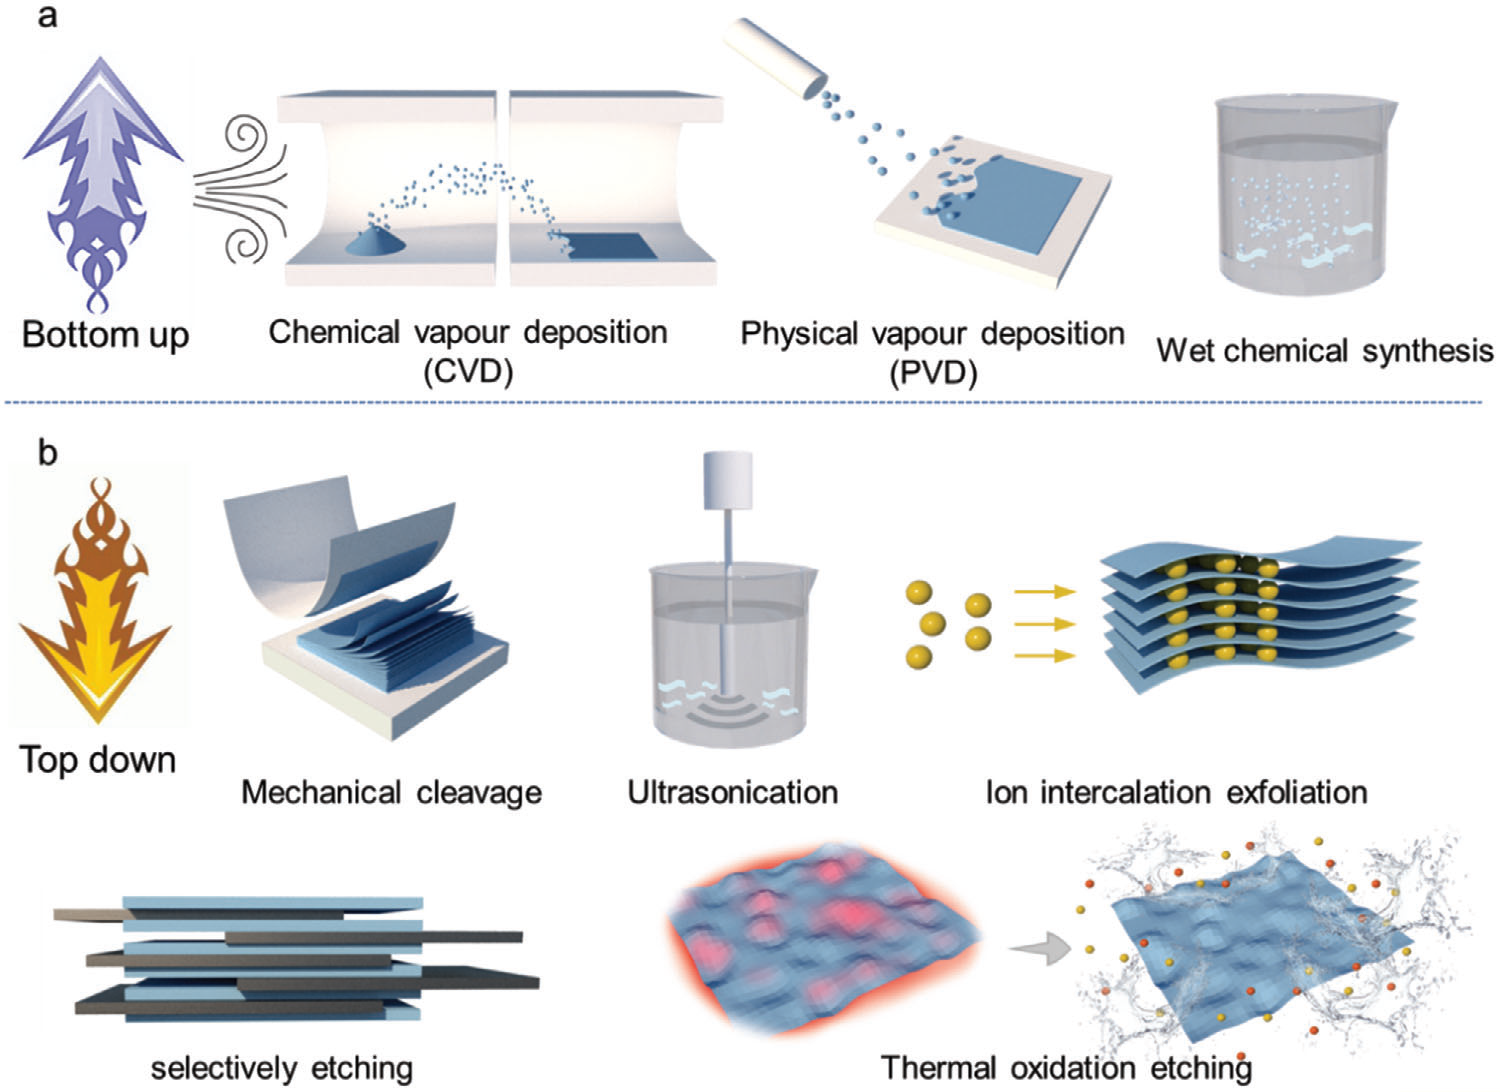
\includegraphics[width=\linewidth]{synthesis.png}
    \caption{روش سنتز اصلی نانوصفحات دو بعدی الف) روش پایین به بالا: CVD، PVD، و مواد شیمیایی مرطوب. ب) روش بالا به پایین: برش مکانیکی، فراصوت، لایه برداری بین یونی، اچ کردن انتخابی، و اچ اکسیداسیون حرارتی.}
    \label{fig:borosynthesis}
\end{figure*}
تکنیک‌های «پایین به بالا» و «بالا به پایین» دو روش اصلی برای تهیه نانومواد دو بعدی هستند. رویکرد "پایین به بالا" شامل رسوب فیزیکی بخار \lr{(PVD)}، \cite{parkCrystallizationInducedPropertiesMorphologyControlled2014, zhaoPatternedGrowthVertically2010, zhaoVerticalOrganicNanowire2009} رسوب بخار شیمیایی \lr{(CVD)}،\cite{zhangReviewChemicalVapor2013, akhavanToxicityGrapheneGraphene2010} [58-65] و روش های سنتز شیمیایی مرطوب، \cite{hanSynthesisStructuralTransformations2013, wuWelldefinedBiOClColloidal2015}[66-69] در میان دیگران است (شکل \ref{fig:borosynthesis} \lr{2a}). \cite{mannixSynthesisChemistryElemental2017}[70] \lr{CVD} شامل تشکیل یک لایه روی یک بستر از طریق پیش سازهای فاز گاز مربوطه است که روی آن واکنش می دهند. محیط، بسترها و پیش سازها سه عامل بسیار مهم بر خواص و رشد محصولات در این روش هستند. اکسیدهای فلزی، گرافن و \lr{h-BN} همگی توسط \lr{CVD} سنتز شده‌اند. در طول فرآیند \lr{PVD}، منبع ماده از طریق روش فیزیکی در شرایط خلاء به حالت گازی تبخیر می‌شود و روی یک بستر رسوب می‌کند تا یک فیلم کاربردی تشکیل دهد. "
ورقه های نانو دو بعدی از مواد بدون لایه اغلب توسط واکنش های شیمیایی در محلول تهیه می شوند که سنتز شیمیایی مرطوب نامیده می شود. بسیاری از مواد مانند\lr{\ch{CuS}}، \lr{\ch{Co3O4}}، $\alpha$-\lr{\ch{Fe2O3}}، \lr{\ch{WO3}} و \lr{Rh} با این روش پربازده و کم هزینه تهیه شده اند. به طور کلی، رویکردهای پایین به بالا را می توان برای سنتز تقریباً همه انواع نانومواد دو بعدی استفاده کرد. رویکردهای "بالا به پایین" شامل برش مکانیکی، \cite{liPreparationApplicationsMechanically2014, yiReviewMechanicalExfoliation2015}[71،72] فراصوت، \cite{nicolosiLiquidExfoliationLayered2013}[73] لایه برداری بین یونی، \cite{yuwenRapidPreparationSinglelayer2016, zengSingleLayerSemiconductingNanosheets2011}[74-77] و اچینگ \cite{anasoriTwoDimensionalOrderedDouble2015, naguibNewTwoDimensionalNiobium2013, naguibTwoDimensionalNanocrystalsProduced2011}[78-80] (شکل \lr{2b}) است. شکاف مکانیکی به نیروهای برشی برای غلبه بر نیروهای واندروالس بین لایه‌های اتصال متکی است و به طور گسترده در لایه‌برداری مواد دو بعدی از مواد حجیم استفاده می‌شود. 8
فراصوت بسته به نیروهای برشی باعث لایه برداری مایع می شود. انرژی صوتی آن می تواند مواد لایه ای مانند گرافیت و \ch{MoS2} را جدا کند. در این روش می توان اندازه، کیفیت و پراکندگی مواد دو بعدی را با حلال فراصوت و زمان کنترل کرد. مزایای استفاده از اولتراسونیک هزینه کم و مقیاس تولید بزرگ است، اما بازده مواد دو بعدی تک لایه کم است. در طول لایه برداری یونی، یون‌ها در فاصله لایه‌ها قرار می گیرند تا نیروهای واندروالس بین لایه‌ها را کاهش دهند و باعث ایجاد لایه برداری شوند. مواد لایه ای، از جمله دی کالکوژنیدهای فلزات واسطه \ch{(TMDs)} و گرافیت، می توانند به راحتی با این روش لایه برداری شوند. روش‌های بالا به پایین ذکر شده در بالا عمدتاً برای جامدات واندروالسی مناسب هستند، در حالی که روش‌های اچ مانند اچ اسید و اچ اکسیداسیون حرارتی معمولاً در جامدات غیر واندروالسی استفاده می‌شوند. اچینگ و لایه برداری انتخابی برای تهیه مواد دو بعدی با پیوند بین لایه ای قوی در مواد حجیم آنها استفاده می شود که با لایه برداری مکانیکی ساده نمی توان به دست آورد. ماده دو بعدی \lr{Mxene} را می توان از طریق اچ کردن انتخابی لایه های \lr{A MAX} (پیش ساز \lr{Mxene}) توسط \lr{HF} بدست آورد. در فرآیند اچینگ اکسیداسیون حرارتی، ماده در دمای بالا به سرعت اکسید می شود و اکسیدهایی را روی سطح تشکیل می دهد که در هوا یا آب ناپایدار هستند. بنابراین، مواد موجود در سطح مواد را می توان از طریق اکسیداسیون و لایه برداری چندگانه اکسید کرد و نانو ورقه‌ها را به دست آورد.
\begin{figure*}[!ht]
    \centering
    \includegraphics[width=\linewidth]{characterizborophene.png}
    \caption{سنتز و خصوصیات بوروفن الف) شماتیک سنتز بوروفن روی نقره. الف) ه است ساختار بوروفن که توسط کامپیوتر پیش بینی شده است. c–h) تصاویر حلقه بسته dI/dV از بوروفن در سمت راست و توپوگرافی STM در مقیاس بزرگ بوروفن در سمت چپ، نمایش کم (c,d)، متوسط ​​(e,f) و بالا (g,h) پوشش. علامت های آبی، قرمز و سفید به ترتیب نشان دهنده نانوروبان های فاز راه راه، جزایر فاز راه راه و فاز همگن هستند. i) تصاویر STM در مورد ساختار سطح اتمی فاز راه راه. شبکه مستطیلی که در تصویر نشان داده شده است بردارهای شبکه را پوشانده است. j) پیکان ارغوانی و لوزی سفید به ترتیب نشان دهنده الگوهای مویره لانه زنبوری و لوزی شکل در فاز راه راه هستند. ک) رشد حالت فرش با جزیره فاز راه راه نشان داده شده است. تصویر نشان می‌دهد که اتم‌های روی مرحله Ag (111) پیوستگی دارند. ج-ک) [36] STM شبیه سازی شده از ورق β12. m) تصویر STM در مورد بوروفن روی بستر Ag (111). n) تصویر سه بعدی از (m) و نوارهای 1.5 نانومتری را می توان به وضوح دید. o) تصویر STM با وضوح بالا در مورد فازهای S1. ص) تصویر STM شبیه سازی شده در مورد ورق χ3. q) تصویر STM از بوروفن روی Ag (111) (650 K); بیشتر جزایر بوروفن از فاز S1 به فاز S2 تبدیل می شوند. r) تصویر STM از ناحیه (f) (با مستطیل برجسته کنید). s) تصویر STM با وضوح بالا در مورد (r) ("S2"). l–s) تکثیر با اجازه.[13] حق چاپ 2016، Springer Nature. t-w) تصاویر STM با وضوح بالا برای P1-P4 نانوروبان های بور در Ag (110)، به ترتیب. t–w)}
    \label{fig:charecterboro}
\end{figure*}
بوروفن و \ch{g}-\ch{C3N4} با این روش با موفقیت تهیه شدند.
\subsection{سنتز پایین به بالا}
\subsubsection{سنتز بر روی \lr{Ag(111)} }
در سال 2015، \lr{Guisinger} و همکاران.\cite{mannixSynthesisBorophenesAnisotropic2015}[36] بوروفن لایه تک اتمی فوق نازک با موفقیت روی نقره تمیز در دمای بین 723 تا 973 کلوین، تحت شرایط خلاء فوق العاده بالا با استفاده از بخار بور سنتز شد (99.9999 درصد خلوص، شار بور در 0.01 تا 0.1 تک لایه در دقیقه به عنوان \lr{[$ML min^{-1}]$} کنترل می شود). منبع بور (شکل \ref{fig:charecterboro}\lr{3a,b}). منبع با خلوص بالا اتم‌های بور از استفاده از پیش‌سازهای سمی (مانند دی‌بوران) اجتناب می‌کند و بستر نقره تمیز، سطح بی‌اثر خوبی برای رشد بوروفن فراهم می‌کند. این روش منجر به تشکیل دو فاز بوروفن شد. فاز همگن و فاز راه راه بیشتر روی نقره در دمای 820 کلوین شکل گرفت (شکل \ref{fig:charecterboro}\lr{3c,d}). دما و نرخ رسوب هر دو بر غلظت‌های نسبی دو فاز تأثیر می‌گذارند، که در آن نرخ‌های رسوب پایین به نفع تولید فاز راه راه هستند در حالی که نرخ‌های رسوب بالاتر به نفع تولید جزایر همگن هستند (شکل \ref{fig:charecterboro}\lr{3c-h}). علاوه بر این، تشکیل فاز راه راه ارتباط نزدیکی با دما داشت، با حداقل حضور این فاز در 720 کلوین و یک فاز تقریباً منحصراً راه راه در 970 کلوین (ساختار در مقیاس اتمی و حالت رشد فاز راه راه در شکل \ref{fig:charecterboro}\lr{3i-k} نشان داده شده است.). نویسندگان همچنین ماده بوروفن لایه تک اتمی فوق نازک را با طیف‌سنجی الکترونی اوگر \lr{(AES)}، میکروسکوپ تونلی روبشی \lr{(STM)} و میکروسکوپ الکترونی عبوری روبشی تصحیح شده با انحراف \lr{(AC-STEM)} در این مطالعه توصیف کردند و نشان دادند که بوروفن دارای خواص فلزی در طول جهت نوار و شکاف باند در امتداد جهت چین خارج از صفحه، همانطور که بر اساس ساختار نوار محاسبه شده پیشنهاد شده است. بنابراین، بوروفن یک ماده دو بعدی بسیار ناهمسانگرد است که قادر به هدایت الکتریسیته در جهت نوار است. علاوه بر این، به دلیل برهمکنش های قوی بین اتم های بور، مدول یانگ در جهت چروک خارج از صفحه بالاتر از گرافن است و در نتیجه خواص مکانیکی ناهمسانگرد ساختار بوروفن چروکیده ایجاد می شود. بنابراین، احتمالاً بوروفن دوبعدی با خواص فلزی و استحکام مکانیکی بالا نقش مهمی در کاربردهای مرتبط دارد. در همین دوره وو و همکاران.\cite{fengDirectEvidenceMetallic2016}[13] بوروفن لایه تک اتمی را روی بستر \lr{Ag(111)} با استفاده از بور با خلوص \lr{99.9999\%} به عنوان منبع بور تحت شرایط خلاء فوق‌العاده رشد داد.

دو فاز بوروفن به نام‌های \lr{S1} (شکل \ref{fig:charecterboro}\lr{3l-o}) و \lr{S2} (شکل \ref{fig:charecterboro}\lr{3p-s})، مطابق با پیش‌بینی‌های نظری $\beta_{12}$ و $\chi_{3}$ مشاهده شد. هر دوی این فازها دارای شبکه های مثلثی بودند، البته با ترتیب متفاوت سوراخ های تناوبی. علاوه بر این، دما بر تشکیل بوروفن تأثیر گذاشت - فازهای \lr{S1} و \lr{S2} ترجیحاً به ترتیب در دمای 570 و 650 کلوین تشکیل شدند، در حالی که بین 650 و 800 کلوین، فازهای \lr{S1} و \lr{S2} با هم وجود داشتند. علاوه بر این، زمانی که پوشش بور به یک تک لایه نزدیک شد، خوشه های بور سه بعدی شروع به شکل گیری کردند، که نشان می دهد برهمکنش بور-نقره نقش مهمی در رشد بوروفن تک لایه ایفا می کند. در سال 2017، پس از به دست آوردن موفقیت آمیز بوروفن در \lr{Ag(111)}، چن و وو و همکاران.[81] نانو نوارهای بوروفن با کیفیت بالا و یکنواختی خوب \lr{(BNRs)} روی \lr{Ag(110)} با عرض متمرکز در حدود 10 نانومتر در دمای 570 کلوین سنتز شد. چهار فاز روی \lr{BNR} وجود دارد که عبارتند از \lr{P1}، \lr{P2}،\lr{P3} و \lr{P4}. سلول های واحد \lr{P1} و \lr{P4} هر دو مستطیلی هستند. مدل‌های اتمی آن‌ها را می‌توان به ترتیب با $\chi_3$ و $\beta_8$ ورق با ثابت‌های شبکه a = 0.40 نانومتر، $b = 0.43$ نانومتر برای \lr{P1} و $a = 0.89$ نانومتر، $b = 0.77$ نانومتر برای \lr{P4} توضیح داد (شکل \ref{fig:charecterboro}\lr{3t}) . سلول واحد \lr{P2} و \lr{P3} لوزی هستند. هر دوی آنها را می توان با مدل ساختار $\beta$، با ثابت های شبکه $a = 0.44$ نانومتر، $b = 0.82$ نانومتر برای \lr{P2} و $a = 0.45$ نانومتر، $b = 0.76$ نانومتر برای \lr{P3} توضیح داد (شکل \ref{fig:charecterboro}\lr{3v,w}). با این حال، ساختارهای ذکر شده در بالا همگی بر اساس زنجیره‌های بور هستند که ممکن است انحراف داشته باشند، و به منظور درک دقیق‌تر ساختار \lr{BNPs}، \lr{Chen} و \lr{Wu} و همکاران. یک نماد جدید، \lr{BC (n, m)} طراحی کرد که در آن مقادیر اتم‌ها در یک زنجیره بور با \lr{m} (باریک‌ترین مناطق) و \lr{n} (عریض‌ترین مناطق) تعریف می‌شوند. با توجه به این نماد، \lr{(P2، P3)}، $\chi_3$ \lr{(P1)} و $\beta_{8}$ \lr{(P4)} را می توان به ترتیب \lr{BC(3،4)}، \lr{BC(2،2)}، و \lr{BC(4،4}) توصیف کرد.
\begin{figure*}[!ht]
    \centering
    \includegraphics[width=\linewidth]{cvdboro.png}
    \caption{}
    \label{fig:cvdboro}
\end{figure*}
\subsubsection{سنتز روی \lr{Cu (111)}}
وانگ و همکاران.\cite{taiSynthesisAtomicallyThin2015}[82] برای سنتز بوروفن از یک دیگ بخار دو بخشی \lr{CVD} خانگی استفاده کرد (شکل \ref{fig:cvdboro} \lr{4a}). قبل از سنتز بوروفن، فویل مسی (ضخامت 25 میکرومتر) در \lr{T2} تا 1237 کلوین گرم شد تا مرزهای دانه بزرگتر شود و سطح فویل مسی صاف شود. پس از آن، منطقه \lr{T1} روی \lr{1337 K} تنظیم شد و \ch{B} $(99.99٪)$ و \ch{2B3O} $(99.98٪)$ در نسبت 1:1 در \lr{T1} برای تولید بخار \ch{2B2O} قرار گرفتند. در نهایت، هیدروژن بخار \ch{2B2O} را به منطقه \lr{T2} منتقل کرد و بوروفن روی فویل مسی تشکیل شد. ساختار بوروفن سنتز شده با روش فوق یک شبکه سه بعدی متشکل از دمبل های \ch{2B} و \ch{12B} ایکو وجهی بود (شکل \ref{fig:cvdboro}\lr{4b,c}). تصاویر نوری بوروفن نشان داد که فیلم بزرگ و پیوسته است (شکل \ref{fig:cvdboro}\lr{4d,e}). میکروسکوپ نیروی اتمی \lr{(AFM)} (شکل \ref{fig:cvdboro}\lr{4f}) و تصاویر میکروسکوپ الکترونی عبوری \lr{(TEM)} (شکل \ref{fig:cvdboro}\lr{4g}) ضخامت لبه تاشو بوروفن 0.80 نانومتر را نشان می دهد که نشان می دهد فیلم از یک لایه تشکیل شده است. تصاویر میکروسکوپ الکترونی عبوری با وضوح بالا \lr{(HRTEM)} نشان داد که بوروفن حاوی یک نوار طولی 1 بعدی متشکل از دو صفحه شبکه قابل انتخاب با گام 0.923 نانومتر است که نشان می‌دهد ساختار بوروفن دارای ویژگی‌های \lr{Pnnm} است. ساختار شبکه بوروفن با تبدیل فوریه سریع \lr{(FFT)} و تصاویر \lr{HRTEM} آشکار شد (شکل \ref{fig:cvdboro}\lr{4h,i}). با ترکیبی از نتایج مشخص‌سازی فوق با پراش پرتو ایکس تک بلور/پودر و محاسبات اصول اول، نشان داده شد که تک لایه $\gamma$-\ch{28B} (شکل \ref{fig:cvdboro}\lr{4j}) با موفقیت روی مس توسط \lr{CDV} سنتز شد. گذر و همکاران.\cite{wuLargeareaSinglecrystalSheets2019}[83] در سال 2019، بوروفن را به ترتیب روی \lr{Ag (111)} و \lr{Cu (111)} سنتز کرده‌اند و ویژگی‌های سنتزی این دو شرایط و ساختار کریستالی بوروفن را به‌طور سیستماتیک، با ترکیب از ابتدا \lr{DFT}، \lr{STM}، پراش و الکترون کم‌انرژی مورد مطالعه قرار داده‌اند. میکروسکوپ آنها دریافتند که حوزه های بوروفن روی \lr{Ag (111)} در همه شرایط رشد مانند دماهای مختلف بستر، مقیاس نانو را حفظ می کنند. با این حال، حوزه‌های تک‌کریستالی نانومقیاس که تاکنون به دست آمده‌اند، برای ساخت دستگاه‌ها بسیار کوچک هستند، در حالی که هرچه اندازه دامنه تک‌کریستالی بزرگ‌تر باشد، کاربرد بوروفن در دستگاه‌ها مفیدتر خواهد بود.

علاوه بر این، گزارش شده است که مواد زیرلایه فلزی می توانند بر چسبندگی و موج دار شدن فیلم، دینامیک رشد و سایر خواص بوروفن تأثیر بگذارند. آنچه در بالا گفته شد نشان می دهد که مواد بستر فلزی انتخاب شده برای ساخت دستگاه بسیار مهم است. با کمال تعجب، گذر و همکاران. ثابت کرد که \lr{Cu(111)}، کم‌تر از نقره، رسانایی بیشتری نسبت به حوزه‌های بزرگ‌تر در حال رشد در تئوری دارد، و آنها حوزه‌های تک بلوری بزرگی از بوروفن، تا اندازه 100 میکرومتر مربع، روی سطح \lr{Cu(111)} به دست آورده‌اند. \lr{T = 770 K} و با نرخ 0.05 $ML min^{-1. 3.1.3.}$ سنتز بر روی \lr{Al(111)} محاسبات نظری نشان داد که به دلیل عدم وجود الکترون، ساختار اصلی بوروفن یک شبکه فشرده مثلثی متراکم است که با \lr{HH} ‌هاهمراه است و تشکیل یک ساختار بوروفن شش ضلعی لانه زنبوری مشابه ساختار گرافن بسیار زیاد است. دشوار. با این حال، چنین ساختار لانه زنبوری شش ضلعی 2 بعدی منحصربفرد، ساختار نوار فرمیون دیراک را به بوروفن می بخشد، که اثرات کوانتومی موجود در گرافم مانند ظهور اثر هال کوانتومی، فرمیون های بدون جرم و تحرک الکترون بسیار بالا را نشان می دهد. این ویژگی‌ها یک سری از کاربردهای بوروفن، از جمله به عنوان حسگرهای زیستی و نانو مواد الکترونیکی را ترویج می کند. ماده ابررسانای معروف \ce{MgB2} از آرایش متناوب لایه‌های اتمی بور با ساختار لانه زنبوری شش ضلعی و لایه‌های اتمی منیزیم با ساختار بسته‌بندی مثلثی شکل تشکیل می‌شود. علاوه بر این، ابررسانایی آن از جفت شدن الکترون-فونون حاصل می شود که در آن لایه اتمی بور فلزی نقش کلیدی ایفا می کند. بنابراین، سنتز موفقیت‌آمیز بوروفن با ساختار لانه زنبوری از اهمیت ویژه‌ای برخوردار است. وو و همکاران.\cite{liSurfaceMorphologyElectrical2018}[84] به یک پیشرفت بزرگ در سنتز بوروفن با ساختار لانه زنبوری شش ضلعی مسطح که مدت‌ها در انتظار بودیم دست یافت. بوروفن لایه تک اتمی بر روی یک بستر \lr{Al (111)} با استفاده از بخار بور با خلوص 99.\lr{9999٪} در شرایط خلاء فوق‌العاده با نرخ رسوب 0.1 میلی‌لیتر در دقیقه (دما: \lr{500 K}) رشد کرد. اتم‌های بوروفن معادل به نظر می‌رسند، که نشان می‌دهد شبکه لانه زنبوری به صورت موضعی صاف بوده است (شکل \ref{fig:cvdboro}\lr{4k,l,n,q,r}). با این حال، شبکه های لانه زنبوری همپوشانی دارند، با راه راه اتمی کمتر از 1.5 بعد از ظهر در دوره بزرگ (شکل \ref{fig:cvdboro}\lr{4m}). منحنی های $dI/dV$ آن نشان داد که ساختار لانه زنبوری شش ضلعی بوروفن دارای خواص فلزی است (شکل \ref{fig:cvdboro}\lr{4o}). علاوه بر این، منحنی $dI/dV$ شکل $V$ نشان داد که ساختار لانه زنبوری شش ضلعی بروفن دارای انرژی فرمی شیب مشابه با نوارهای دیراک مشخصه گرافن است (شکل \ref{fig:cvdboro}\lr{4p}). 
\begin{figure*}
    \centering
    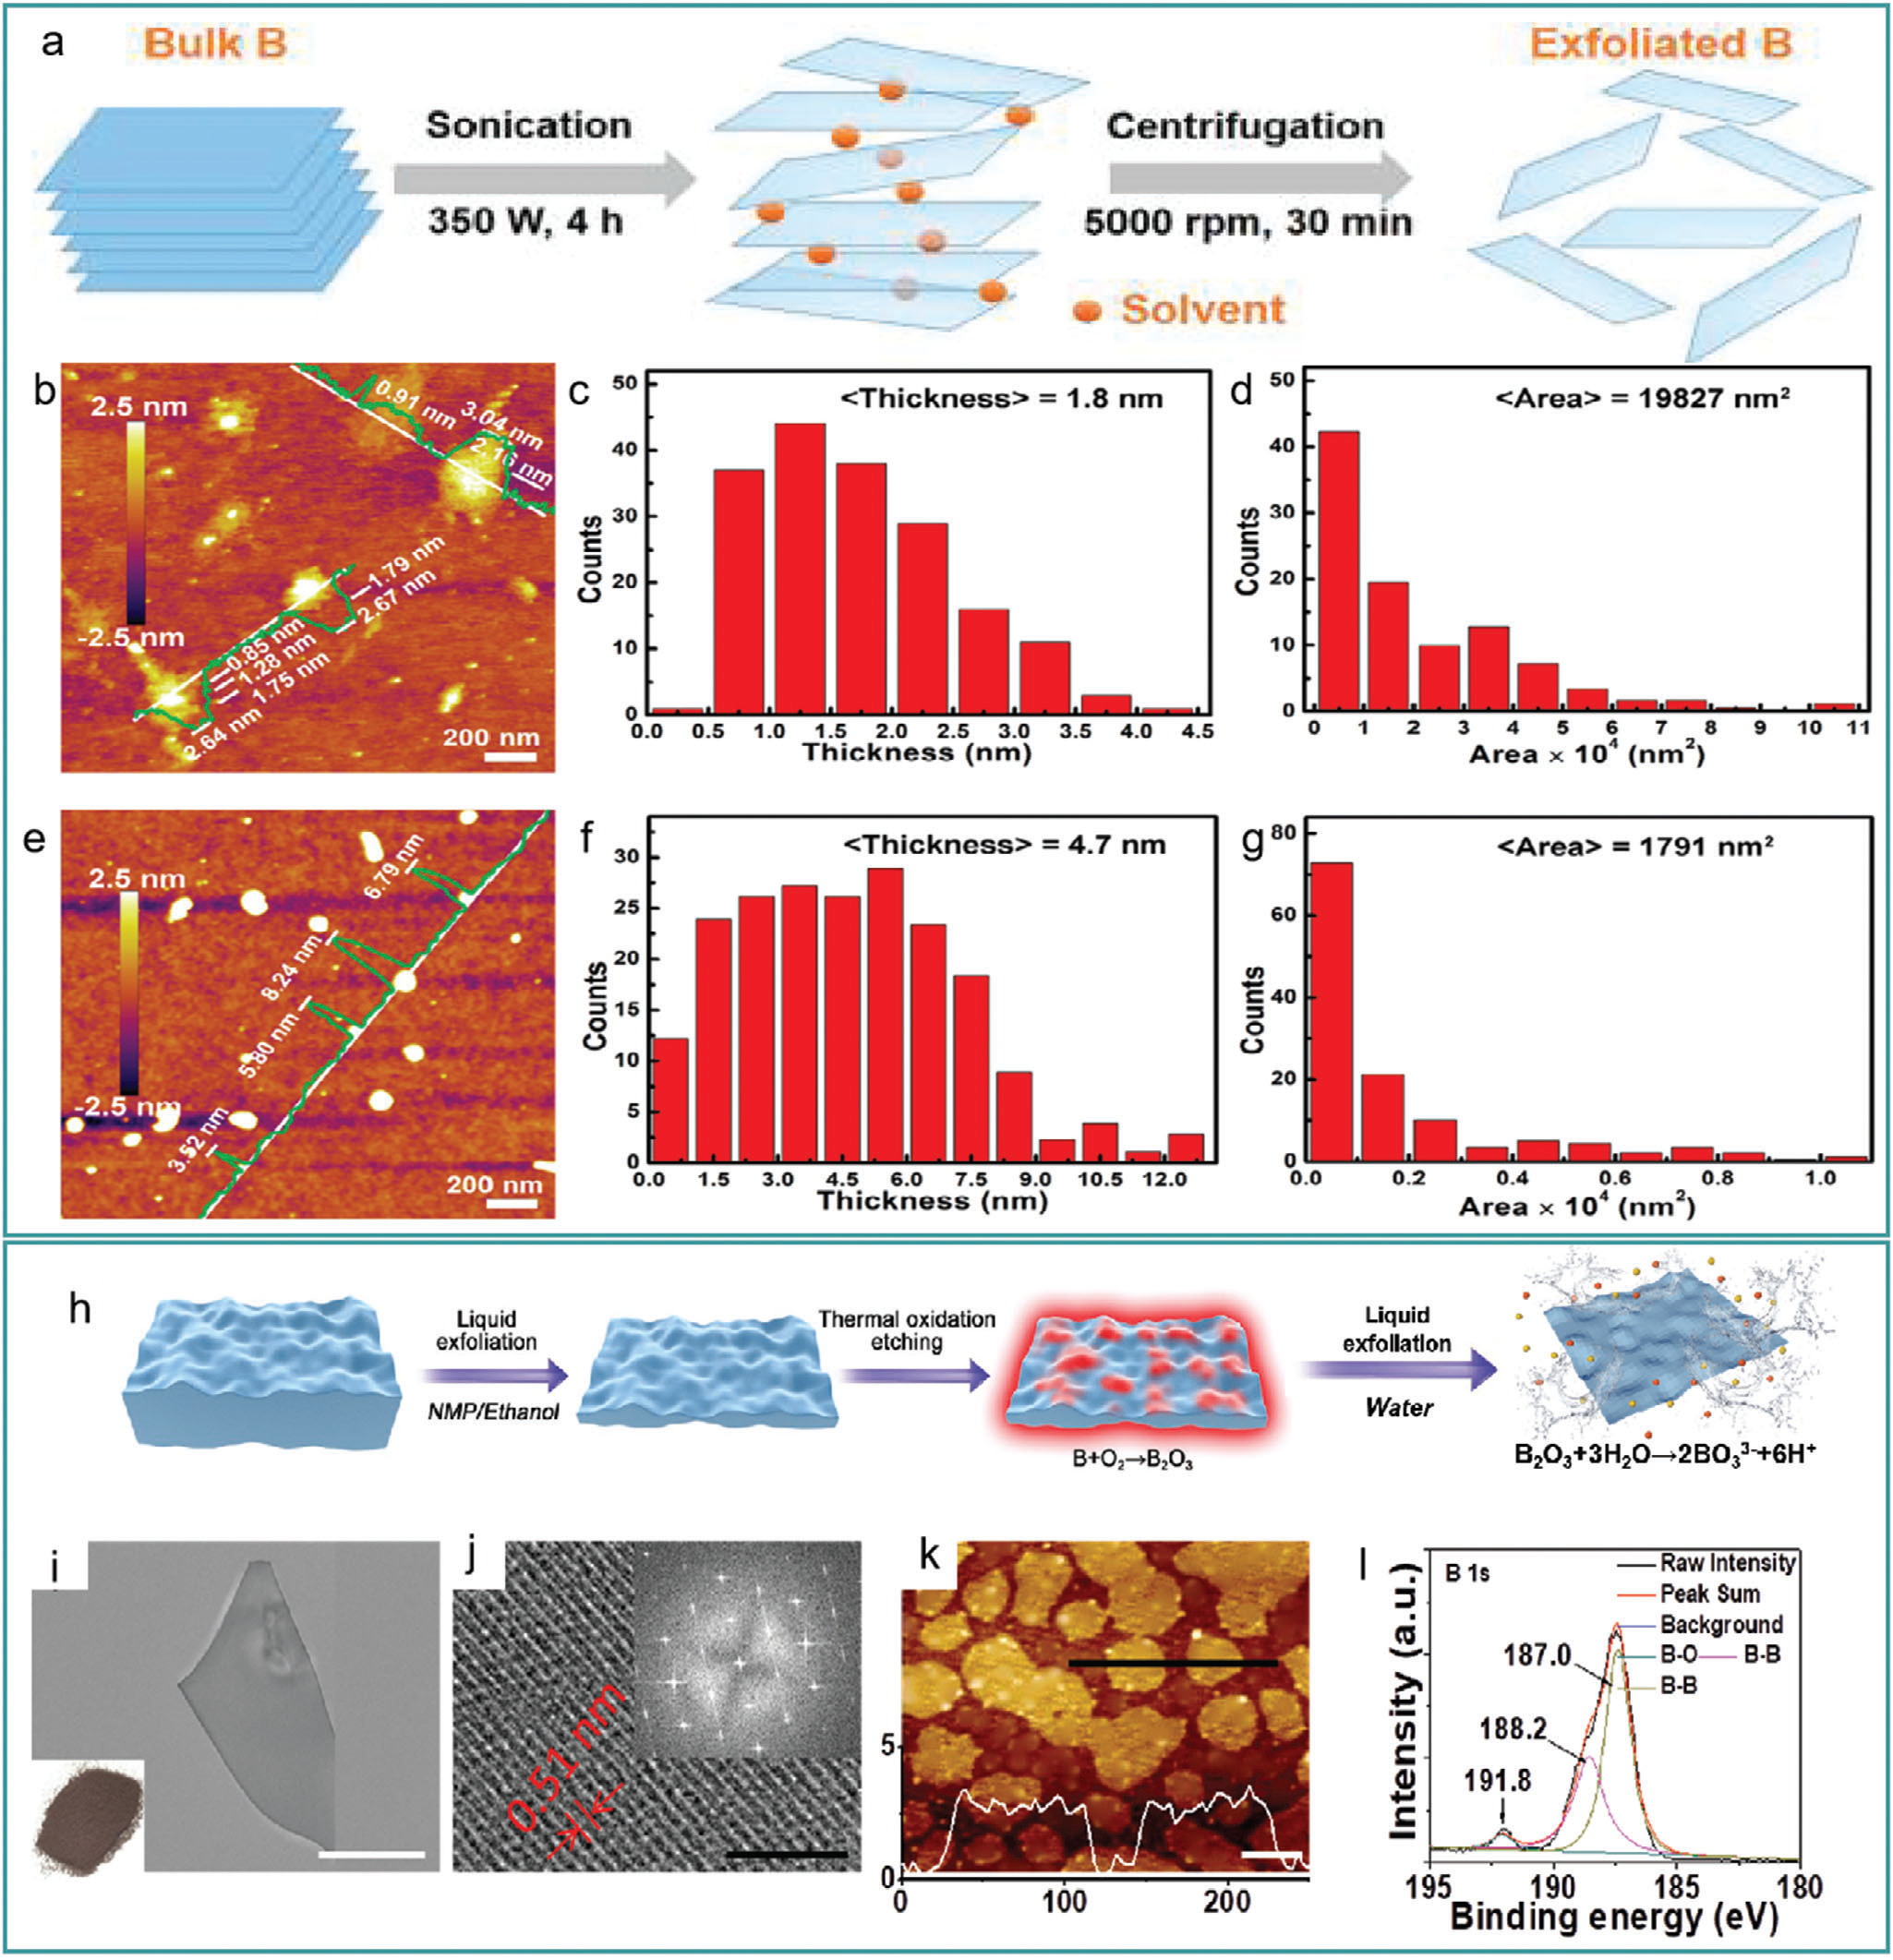
\includegraphics[width=\linewidth]{AFM.png}
    \caption{الف) شماتیک سنتز لایه برداری فاز مایع بوروفن های با کیفیت بالا به کمک فراصوت. b-g) خصوصیات AFM بوروفن سنتز شده در DMF (b-d) و IPA (e-g) توسط فراصوت. ب، ه) تصاویر توپوگرافی AFM و مشخصات ارتفاع. c,f,d,g) ضخامت و اندازه بوروفن آماده شده. الف – ز) تکثیر با اجازه.[86] حق چاپ 2018، انجمن شیمی آمریکا. ح) شماتیک اچینگ اکسیداسیون حرارتی و سنتز لایه برداری مایع بوروفن. i-l) تصاویر TEM، HRTEM، AFM، و طیف XPS بوروفن که با لایه برداری مایع در آب سنتز می شوند. نوار مقیاس سفید = 100 نانومتر و نوار مقیاس سیاه = 5 نانومتر. h–l) با اجازه تکثیر شده است.[25] حق چاپ 2018، Wiley-VCH.}
    \label{fig:afm}
\end{figure*}
\subsubsection{سنتز روی \lr{Au (111)}}
اخیراً \lr{Guisinger} و همکاران.\cite{kiralyBoropheneSynthesisAu2019}[85] بوروفن را با موفقیت روی یک زیرلایه \lr{Au(111)} سنتز کرد و تأثیر زیرلایه‌های \lr{Au(111)} با دمای متفاوت را بر رسوب حرارتی اتم‌های بور بررسی کرد. تصاویر \lr{SEM} از تمیز \lr{Au(111)} و بوروفن سنتز موفقیت آمیز بوروفن روی طلا را نشان دادند (شکل \ref{fig:cvdboro}\lr{4u,v}). بر خلاف سنتز بوروفن بر روی سوبستراهای \lr{Ag(111)}، \lr{Cu(111)} و \lr{Al(111)}، در زیرلایه \lr{Au(111)}، اتم های بور ابتدا در اتم های طلا در دماهای بالا (برابر یا بیشتر از 823 کلوین) حل می شوند. پس از سرد شدن به سطح جدا می شود و بوروفن را تشکیل می دهد (شکل \ref{fig:cvdboro}\lr{4s}). در فرآیند سنتز بوروفن بر روی یک زیرلایه \lr{Au(111)}، جزایر بورفن نانومقیاس بر روی سطح Au(111) مشاهده شد (شکل \ref{fig:cvdboro}\lr{4v})، که از 1 تا 8 ساختار لوزی شکل 1 نانومتر مربع در مساحت سطح با یک بوروفن تشکیل شده است. 12 ساختار اتمی و هدایت فلزی (شکل \ref{fig:cvdboro}\lr{4t,w}). با افزایش غلظت بور، شبکه سه ضلعی شکسته شد و جزایر بوروفن بزرگتری را در سطح بستر تشکیل داد (شکل \ref{fig:cvdboro}\lr{4x}). بنابراین، بر اساس مطالعات فعلی، هرچه غلظت اتم بور بزرگتر باشد، اندازه بوروفن بزرگتر است. با این حال، کاربردهای بیشتر بوروفن به دلیل دشواری انتقال بوروفن از بسترهای فلزی محدود است.

با توجه به پیوندهای ضعیف و انتقال بار محدود بین \lr{Au (111)} و بوروفن تشکیل شده بر روی سطح، بوروفن به راحتی جدا می شود که امکان کاربرد بیشتر را فراهم می کند. با این حال، تنها چند گزارش در مورد سنتز بوروفن در آزمایشگاه موجود است. همه نمونه‌های بالا از سنتز موفق بورفن که تاکنون گزارش شده‌اند شامل روش‌های پایین به بالا هستند، به جز دو گزارش از سال 2018، که در آنها از روش‌های بالا به پایین استفاده شده است، همانطور که در زیر توضیح داده شده است.
\subsection{سنتز بالا به پایین}
تئو و همکاران.\cite{liScalableProductionFewLayer2018}[86] ثابت کرد که بوروفن چند لایه با کیفیت بالا با اندازه و ضخامت کنترل شده را می توان با لایه برداری فاز مایع به کمک اولتراسونیک سنتز کرد. در طول فرآیند سنتز، پودر بور در یک حلال دی متیل فرمامید \lr{(DMF)} / ایزوپروپیل الکل \lr{(IPA)} (1 میلی گرم در میلی لیتر) پراکنده شد و به مدت 4 ساعت در 350 وات فراصوت شد. بوروفن با ضخامت های مختلف با تنظیم سرعت سانتریفیوژ جمع آوری شد (شکل \ref{fig:afm}\lr{5a}). پس از آن، بوروفن به دست آمده توسط \lr{AFM} مشخص شد (شکل \ref{fig:afm}\lr{5b,e}). بوروفن جدا شده در \lr{DMF} دارای ضخامت متوسط 1.8 نانومتر و مساحت 19827 نانومتر بود (شکل \ref{fig:afm}\lr{5c,d})، در حالی که بوروفن جدا شده در \lr{IPA} دارای ضخامت 4.7 نانومتر و مساحت 1791 نانومتر بود (شکل \ref{fig:afm}\lr{5f,g}). بنابراین، اندازه و ضخامت بوروفن را می توان با تنظیم حلال مورد استفاده در لایه برداری اولتراسونیک کنترل کرد. جی و همکاران با الهام از خواص شیمیایی ویژه بور، که در آن بوروفن بی اثری در مقابل اکسیداسیون نشان می دهد، در حالی که لبه بیرونی آن و بور توده ای سه بعدی هر دو به راحتی اکسید می شوند.\cite{jiNovelTopDownSynthesis2018}[25] روش دیگری برای سنتز از بالا به پایین با استفاده از اچینگ در دمای بالا و سلب فاز مایع ایجاد کرد. پودر بور در یک حلال N-متیل پیرولیدون \lr{(NMP)} و الکل 1:1 پراکنده شد و به مدت 5 ساعت در 500 وات اولتراسونیک شد. سپس، ورقه های بور جدا شده و در یک ظرف سرامیکی حاوی اکسیژن در دمای 923 کلوین قرار داده شدند تا سطح دانه های بور به \ch{2B3O} اکسید شود. متعاقبا، از روش لایه برداری فاز مایع برای حل شدن سطح \ch{2B3O} در \ch{B3O} 3- استفاده شد (شکل \ref{fig:afm}\lr{5h}). در نهایت، بوروفن با اندازه مسطح ≈110 نانومتر و ضخامت کمتر از 3 نانومتر به دست آمد (شکل \ref{fig:afm}\lr{5i,k}). بوروفن حاوی حاشیه‌های تداخلی بود و گام راه راه آن 0.51 نانومتر بود که با ویژگی‌های ساختار بور $\beta$-لوزی وجهی مطابقت داشت (شکل \ref{fig:afm}\lr{5j}). طیف \lr{XPS} بوروفن (شکل \ref{fig:afm}\lr{5l}) سنتز موفقیت آمیز بوروفن را پس از لایه برداری لایه های اکسید شده در آب تایید کرد. این کار اولین گزارشی است که در مورد سنتز توده‌های بور به بوروفن با روشی از بالا به پایین بحث می‌کند، سطح ویژه بوروفن را تا حد زیادی بهبود می‌بخشد و کاربرد آن در دارورسانی را بهبود می‌بخشد. 3.3. عوامل کلیدی در سنتز بوروفن بر اساس نتایج تحقیقات نظری و سنتز تجربی، بستر، دما و حلال به عنوان عوامل کلیدی موثر بر تشکیل بوروفن نشان داده شده است. در ادامه، این عوامل کلیدی را به تفصیل تجزیه و تحلیل خواهیم کرد.

\subsection{تأثیر بستر فلزی بر سنتز بوروفن}
نظریه هسته‌زایی کلاسیک نشان می‌دهد که سد انرژی هسته‌زایی تشکیل مواد را تنظیم می‌کند، در حالی که مانع هسته‌زایی بور 2 بعدی بالاتر از ساختار توده‌ای سه بعدی آن است و از هسته‌زایی طبیعی بوروفن جلوگیری می‌کند.\cite{liuProbingSynthesisTwoDimensional2013, piazzaPhotoelectronSpectroscopyInitio2012, sergeevaB22B23AllBoron2012, kiranPlanartotubularStructuralTransition2005, ogerBoronClusterCations2007}[87-91] نقص‌های ترمودینامیکی. و پلی مورفیسم بوروفن دشواری سنتز آن را افزایش می دهد. بنابراین، کاهش سد هسته‌زایی بور دو بعدی و القای هسته‌زایی دوبعدی یک مسیر انرژی مطلوب برای سنتز بوروفن است.\cite{liEvolutionGrapheneGrowth2009}[92] در سال 2013، یاکوبسون و همکاران.\cite{liuProbingSynthesisTwoDimensional2013}[87] نشان داد که برهمکنش بین لایه‌های فلزی و بور به هسته‌زایی بورنن کمک می‌کند، زیرا مانع هسته‌زایی سه‌بعدی بور در برخی از بسترهای فلزی بالاتر از دو بعدی است.

چه نوع بستری برای سنتز بوروفن مناسب است؟ دو معیار برای انتخاب زیرلایه‌های فلزی مناسب پیشنهاد شده است: باید حلالیت کمی در اتم‌های بور داشته باشد و نیروی اتصال بین بستر و اتم‌های بور باید متوسط باشد.\cite{liEvolutionGrapheneGrowth2009}[92] اگر نیرو بیش از حد قوی باشد، جدا کردن بوروفن از بستر دشوار است و بوروفن حتی ممکن است به راحتی یک بورید تشکیل دهد. به عنوان مثال، هنگامی که بوروفن بر روی بسترهای آهن، کو، یا نیکل سنتز می شود، \cite{vajeestonElectronicStructureBonding2001, burdettELECTRONICSTRUCTURETRANSITIONMETALBORIDES1986}[93،94] بورید می تواند به راحتی تشکیل شود. علاوه بر این، در زیرلایه های طلا، از آنجایی که برهمکنش بین اتم طلا و بور بسیار ضعیف است، بور غیرمسطح ممکن است به راحتی تشکیل شود.\cite{zhangTwoDimensionalBoronMonolayers2015}[95] با توجه به برهمکنش بین بوروفن و بستر فلزی، بسترهای رایج مورد استفاده را می توان به دو دسته عمده تقسیم کرد: یکی دارای انرژی اتصال قوی و انتقال بار زیاد با بوروفن، از جمله \lr{Mg(0001)}، \lr{Al(111)}، و \lr{Ti(0001)} است. \cite{hyamEffectParticleSize2008, cepekEpitaxialGrowthMgB22004}[96،97] مشخصات نوارهای $\sigma$ (داخلی) بوروفن شش ضلعی سنتز شده روی این بسترها، به جز تغییر سطح فرمی، شبیه به فاز ایستاده آن است. دیگری انرژی پیوند نسبتاً پایین‌تری با بوروفن دارد، از جمله \lr{Au(111)} و \lr{Ag (111)}، و باندهای درون صفحه بوروفن شش ضلعی به زیر باندهای زیادی تقسیم می‌شوند.\cite{zhangBoronSheetAdsorbed2012}[98] خو و همکاران \cite{xuNucleationGrowthBorophene2016}[99] به طور نظری مکانیسم هسته‌زایی و فرآیند رشد بوروفن را در سطح \lr{Ag(111)} ارزیابی کرد و تأیید کرد که ساختار پایدار بهینه، ساختاری است که \lr{HHs} به‌طور موازی مرتب شده‌اند و غلظت \lr{HHs} با آزمایش 1/6 بود. ژائو و همکاران \cite{liuBoronClusterTwoDimensional2013}[100] دریافتند که خوشه های بور متراکم دوبعدی به راحتی روی سطح مس (111) تشکیل می شوند. علاوه بر این، هر چه اندازه خوشه بزرگتر باشد، انرژی تشکیل کوچکتر است. بنابراین، بسترهای فلزی تفاوت زیادی در ساختار بوروفن ایجاد شده ایجاد می کنند و انتخاب یک بستر مناسب با توجه به محصول مورد نظر اهمیت ویژه ای دارد.

\section{خواص بوروفن}
\subsection{خواص شیمیایی}
نشان داده شده است که بور 2 بعدی نسبت به اکسیداسیون بی اثر است، در حالی که لبه بیرونی آن و بور توده‌ای 3 بعدی کمتر است.\cite{fengExperimentalRealizationTwodimensional2016}[13] بور دارای سه الکترون ظرفیتی است \lr{([He]2S22P1)}. با این حال، یک الکترون ارتقا یافته از اوربیتال \lr{2S} به \lr{2P} می تواند بور را قادر سازد که چهار اوربیتال ظرفیتی در دسترس داشته باشد. بنابراین، تعداد الکترون های ظرفیت کمتر از تعداد اوربیتال های ظرفیت است و اوربیتال های الکترونیکی را نمی توان به طور کامل با الکترون های اتم بور در هنگام تشکیل پیوندهای شیمیایی پر کرد و منجر به تشکیل اتم های بور فاقد الکترون می شود. ترکیب اتم‌های بور سه‌بعدی حجیم و اتم‌های اتم‌های بور دو بعدی در اطراف محیط، هر دو بر اساس پیوندهای دو الکترونی کلاسیک دو مرکزی هستند، اما اتم‌های داخلی پیوندهای دو الکترونی چند مرکزی بورونار دوبعدی غیرمحلی شده‌اند که منجر به تفاوت آنها در پایداری اکسیداسیون می‌شود. \cite{zhangTwodimensionalBoronStructures2017}[37] به عنوان مثال، در یک صفحه بور، \lr{HH}‌ها به عنوان "پذیرنده" عمل می کنند و اتم های بور در مرکز شش ضلعی‌ها به عنوان "اهداکننده" عمل می کنند، بنابراین کمبود الکترون در بور را جبران می کنند و ورقه های بور را نسبت به اکسیداسیون بی اثر می کنند.[51] وو و همکاران.\cite{fengExperimentalRealizationTwodimensional2016}[13] از طیف‌سنجی فوتوالکترون پرتو ایکس \lr{(XPS)} برای تشخیص ترکیب شیمیایی بوروفن تک‌لایه استفاده کرد و نشان داد که دو پیک انرژی کم‌پیوند (\lr{188.2 و 187.1} \lr{eV}) از دو پیوند \ch{B-B} مختلف در ورقه‌های بور 2 بعدی هستند، در حالی که اتصال هستند. انرژی بور فله \lr{1s} اوج در بور فله \lr{3D} به طور کلی \lr{≈189-190 eV} است. با این حال، اوج انرژی بالاتر \lr{(191.5 eV)} قرار است از اتم بور اکسید شده ناشی شود، بر اساس پیک های بور اکسید شده قبلا گزارش شده است.
  
از طریق محاسبه و مقایسه مساحت پیک، مشاهده شد که نسبت اتم بور اکسید شده به اتم بور اکسید نشده تنها \lr{23/0 ≈} است که نشان می‌دهد اکثر اتم‌های بور روی سطح بوروفن دارای ثبات خاصی در برابر اکسیداسیون هستند. علاوه بر این، اتم های اکسید شده عمدتاً در لبه فیلم بوروفن قرار دارند که می تواند با آزمایش های \lr{STM} درجا تأیید شود. اکسیژن به طور مستقیم به محفظه خلاء پمپ شد و سطح بور در محل با استفاده از \lr{STM} اسکن شد. در غلظت‌های بالای اکسیژن، لکه‌های روشن در لبه‌های جزیره بور ظاهر می‌شوند که نشان می‌دهد اتم‌های بور شروع به اکسید شدن کرده‌اند، در حالی که تراس ورقه‌های بور تغییر کمی نشان می‌دهد. با ادامه جریان اکسیژن، ورقه‌های بور پایدار ماندند و فاز مخطط هنوز قابل مشاهده بود، که نشان می‌دهد اکسیداسیون بور عمدتاً در لبه‌ها اتفاق می‌افتد، در حالی که ورقه بور خود در برابر اکسیداسیون پایدار است. بنابراین، بوروفن دو بعدی در مقایسه با بور فله سه بعدی نسبت به اکسیداسیون بی اثرتر است. علاوه بر این، \lr{Guisinger} و همکاران.\cite{mannixSynthesisBorophenesAnisotropic2015}[36] همچنین دریافتند که حالت اکسیداسیون در بوروفن زمانی که در معرض شرایط محیطی قرار می‌گیرد تشخیص داده می‌شود، اما اکسیداسیون عمدتاً در لبه‌های بوروفن به دلیل حالت‌های لبه فعال آن رخ می‌دهد. با وجود قرار گرفتن در معرض دوز بالای اکسیژن، مناطق با شبکه کامل تقریبا دست نخورده باقی می مانند.\cite{zhaiObservationAllboronFullerene2014}[103] با این وجود، \lr{Guisinger} و همکاران. همچنین نشان داد که بوروفن به اندازه مواد دوبعدی دیگر از نظر شیمیایی پایدار نیست و زمانی که برای مدت طولانی در معرض هوا قرار می‌گیرد می‌تواند مستعد آلودگی باشد. این پایداری شیمیایی، اگرچه قابل مقایسه با گرافن نیست، به حل مشکل ناپایداری در برابر اکسیداسیون در مواد دو بعدی کمک می کند. علاوه بر این، پایداری بوروفن در برابر اکسیژن را می توان با به عنوان مثال، مهر و موم کردن بوروفن از اکسیژن با پوشاندن مواد دیگر افزایش داد، و همچنین ثابت کردند که یک لایه درپوش اکسید سیلیسیم/سیلیکا می تواند تا حد زیادی مانع اکسیداسیون بوروفن شود که منجر به مطالعه بیشتر ما می شود. در مورد مقاومت اکسیداسیون بور 2 بعدی.\cite{zhangTwodimensionalBoronStructures2017}[37] از سوی دیگر، با فعالیت شیمیایی لبه‌های بوروفن، می‌تواند واکنش‌های تکامل هیدروژن را کاتالیز کند؛ \cite{zhangTwoDimensionalBoronMonolayers2015}[95] این ویژگی جالب نه تنها امکان جدیدی را برای توسعه انرژی جایگزین فراهم می‌کند، بلکه مسیرهای جدیدی را برای کاربرد بور باز می‌کند.

\subsection{ویژگی های مکانیکی}
بوروفن، ساخته شده از پیوندهای کووالانسی چند مرکزی به جای پیوندهای کووالانسی کلاسیک دو مرکزی موجود در سایر مواد دو بعدی معمولی، نوید خواص مکانیکی استثنایی را می دهد. پیوندها یکی از قوی‌ترین پیوندها در طبیعت هستند که منجر به استحکام بسیار بالا در داخل صفحه و پایداری ساختاری عالی گرافن می‌شود. در مورد بوروفن، علاوه بر پیوندهای کووالانسی کلاسیک که استحکام مهمی به ورق می دهد، پیوندهای فلزی مانند چند مرکزی به طور کلی به ساختار سیالیت بالقوه می بخشند.\cite{zhangTwoDimensionalBoronMonolayers2015}[95] بعلاوه، به عنوان یک ماده دو بعدی، بوروفن به دلیل ضخامت اتمی، انعطاف پذیری بسیار خوبی از خود نشان می دهد. علاوه بر این، طبق پیش‌بینی‌ها، بوروفن در یک کرنش بزرگ تحت یک انتقال فاز ساختاری قرار می‌گیرد که منجر به چقرمگی مکانیکی بالاتر می‌شود. علاوه بر این، وانگ و همکاران.\cite{wangStrainEffectsBorophene2016}[109] ثابت کرد که از آنجایی که پیوندهای \lr{B-B} هنگام افزایش کرنش کششی ضعیف می شوند، نسبت پواسون در امتداد جهت خارج از صفحه منفی است.\cite{liuRecentProgressGrapheneanalogous2019}[110] پارامترهای خاص در جدول 2 خلاصه شده است. نشان داده شده است که سفتی درون صفحه 1/6 بوروفن کمتر از بسیاری از مواد دو بعدی مانند گرافن است.\cite{zhangElasticityFlexibilityIdeal2017}[107] محاسبه شد که عدد \lr{Foppl-von Karman} در واحد سطح صفحه \lr{$\nu$=1/6} که به صورت \lr{C/D} تعریف می شود، یعنی نسبت بین مدول درون صفحه و سختی خمشی، در بین مواد ذکر شده بالاترین است. در آن تحقیق بنابراین، یکی از منعطف ترین مواد با سطوح بالایی از انعطاف پذیری در برابر تغییر شکل خارج از صفحه است. بوروفن را می توان بر اساس هندسه اتمی آن، شامل ورق های مثلثی ($\nu_0$)، ورقه های $\alpha$ (1/9)، 1/5، 1/6، 1/7، 1/8، 1/10 و 2 ورق‌ها طبقه بندی کرد. \cite{zhaoPhononmediatedSuperconductivityBorophenes2016}[111] ورق‌های مثلثی شل به دلیل وجود الکترون‌های زیاد، ساختار کمانشی مانند تخته‌شویی را نشان می‌دهند، در حالی که ورقه‌های 1/5، 1/6 و سایر صفحات به دلیل غلظت بالای \lr{HH} که منجر به کمبود الکترون در خلاء می‌شود، کاملاً مسطح هستند. ساختار مسطح ناپایداری ناشی از ساختار کمانش ورق بور مثلثی را حل می کند. همانطور که در بالا ذکر شد، ورود \lr{HHs} به بوروفن می تواند به طور موثر ساختار را تثبیت کند، زیرا کرنش اعمال شده در نزدیکی \lr{HHs} بسیار متمرکز است، که کشسانی کل ورق‌ها را کنترل می کند. از سوی دیگر، افزایش غلظت \lr{HH} می تواند سطح ورق را گسترش دهد، در نتیجه کشش را کاهش می دهد، و انتقال فاز ساختاری تجربه شده توسط بوروفن می تواند مواد را سخت تر کند و در برابر بارهای بزرگ حتی در کشش شدید مقاومت کند. بنابراین، \lr{HH} ها برای فرآیند شکستن انعطاف پذیر بوروفن حیاتی هستند. با این وجود، \lr{HH} ها به طور قابل توجهی بر خواص مکانیکی مواد تأثیر می گذارند. افزایش \lr{HHs} باعث کاهش تعداد پیوندهای \lr{B-B} و در نتیجه سختی مواد می شود. استحکام کششی نهایی شبکه بور نیز به شدت تحت تأثیر قرار خواهد گرفت. به عبارت دیگر، با اضافه کردن HH ها، با وجود افزایش $\eta$، تغییرات سفتی بوروفن محدود می شود. با توجه به روش جابجایی اتمی، \cite{zhangElasticityFlexibilityIdeal2017, schabelENERGETICSINTERPLANARBINDING1992, wangStrainEffectsBorophene2016}[107,109] $\nu=1/6$ پیش‌بینی شده است که دارای استحکام ایده‌آل 16.4 نیوتن متر-1 است – علیرغم اینکه به خوبی برای ورق‌های گرافن و نیترید بور شش ضلعی \lr{(h-BN)} نیست، بالاتر از سایر مواد دو بعدی، مانند \lr{MoS2} \cite{liIdealStrengthPhonon2012, zouPredictingDislocationsGrain2013}[112،113] و فسفرن.\cite{weiSuperiorMechanicalFlexibility2014}[114] علاوه بر این، سفتی خمشی و نسبت پواسون نیز به شدت به چگالی \lr{HH} بستگی دارد. بنابراین، این پارامترهای مکانیکی را می توان به طور انعطاف پذیر با توجه به الزامات برنامه های مختلف تغییر داد.\cite{zhangElasticityFlexibilityIdeal2017}[107] مکانیسم ناپایداری بوروفن نیز ارزیابی شد، \cite{wangStrainEffectsBorophene2016, zhongElectronicMechanicalProperties2018, weiSuperiorMechanicalFlexibility2014, zouPredictingDislocationsGrain2013}[109,115] که نشان می‌دهد مکانیسم شکست، ناپایداری الاستیک تحت یک کرنش تک محوری در جهت زیگزاگ است، در حالی که برای کرنش تک محوری در امتداد جهت صندلی و کرنش دو محوره، مکانیسم شکست به فونون نسبت داده می‌شود. بی ثباتی. بوروفن به عنوان یک ماده دو بعدی با انعطاف پذیری بی سابقه، استحکام ایده آل بالا و خاصیت ارتجاعی عالی پتانسیل بالایی در تهیه مواد کامپوزیتی و دستگاه های انعطاف پذیر دارد. این داده‌ها نشان می دهد که خواص بوروفن را می توان با تنظیم غلظت \lr{HHs} و تسلط بر مکانیسم ناپایداری بوروفن تنظیم کرد.

\section{خواص الکتریکی}
با ماهیت کمبود الکترون عنصر \lr{B}، پایدارترین ساختار مخلوطی از ساختارهای شش ضلعی و مثلثی \cite{tangNovelPrecursorsBoron2007}[52] با پیوندهای دو و سه مرکز است. دارای خواص الکتریکی نسبتا منحصر به فردی مانند فلزی بودن، اثرات دیراک فرمی، ابررسانایی و نیمه رسانایی است
\section{فلزی بودن}
یاکوبسون و همکاران.\cite{penevCanTwoDimensionalBoron2016}[120] از نظر تئوری پیش‌بینی شد که همه پلی‌مورف‌های بوروفن فلزی هستند، متفاوت از خواص نیمه‌رسانا یا عایق آلوتروپ‌های توده‌ای سه‌بعدی، که تنها بخش کوچکی از آن‌ها می‌توانند تحت فشار فوق‌العاده به فلز تبدیل شوند.\cite{eremetsSuperconductivityBoron2001}[121] پس از آن، به طور تجربی تایید شد که فلزی بودن توسط مدار $p_z$ تعیین می‌شود.\cite{shangTwoDimensionalBoron2018}[39] وو و همکاران.\cite{fengExperimentalRealizationTwodimensional2016}[13] از طیف‌سنجی تونلی روبشی برای اندازه‌گیری حالت‌های الکترونیکی فازهای 12 و 3 با موفقیت استفاده کرد و دریافت که چگالی‌های محلی حالت‌ها در اطراف سطح فرمی وجود دارد که ساختار نوار انرژی فلزی بودن را بیشتر نشان می‌دهد. ماتسودا و همکاران.\cite{fengDirectEvidenceMetallic2016}[122] باندهای مشتق از بور فلزی $\beta_{12}$ را با استفاده از طیف‌سنجی فوتوالکترون با تفکیک زاویه مشاهده کرد و یک پدیده جالب را استنباط کرد - همزیستی پاکت‌های الکترونیکی و حفره‌های حفره‌ای در سطح فرمی - طبق محاسبات اولیه اولیه، که فلزی بودن آن را نیز نشان می‌دهد. علاوه بر این، \lr{Fazzio} و همکاران.\cite{padilhaDirectionalDependenceElectronic2016}[123] تایید کرد که رسانایی بوروفن ناهمسانگرد است و انتقال جریان در دو جهت عمود بر هم وابسته است.
\subsection{خواص توپولوژیکی}
مواد توپولوژیکی بسیاری از خواص کوانتومی جدید متفاوت از مواد سنتی را نشان می‌دهند، \cite{qiTopologicalInsulatorsSuperconductors2011}[124] و با توجه به ساختارهای الکترونی می‌توان آنها را به سه نوع تقسیم کرد، یعنی عایق‌های توپولوژیکی، \cite{hsiehTopologicalCrystallineInsulators2013}[125] نیمه فلزی ویل توپولوژیکی، \cite{xuDiscoveryWeylFermion2015}[126] و نیمه فلزی دیراک توپولوژیکی. \cite{wanTopologicalSemimetalFermiarc2011}[127] نیمه فلز دیراک توپولوژیکی ساختار الکترونی منحصر به فردی را نشان می دهد که در آن نوارهای انرژی نزدیک به سطح فرمی دارای نقاط دیراک سه بعدی هستند و سه جهت حرکت مجاور اطراف نقاط دیراک همگی روابط پراکندگی خطی هستند. چنین ویژگی‌های عبور نواری توسط تقارن کریستالی محافظت می‌شوند، که باعث می‌شود چشم‌انداز کاربردی بسیار جذابی در دستگاه‌های الکترونیکی، نیمه‌رساناها و سایر زمینه‌ها داشته باشند.\cite{zhaoPalgraphynePromising2D2020}[128] در حالی که مواد دیراک توپولوژیکی کشف شده تا کنون معمولاً حاوی عناصر فلزی سنگین هستند که با مشکلات سختی روبرو هستند که برای کاربردهای عملی رسانا نیستند، به عنوان مثال، آلودگی محیطی، هزینه بالا و ایمنی مواد. بنابراین، بررسی عناصر سبک برای ترکیب مواد توپولوژیکی پایدار ضروری است. گرافن ماده معمولی سبک دیراک است که بسیاری از پدیده های فیزیکی جدید و خواص الکترونی که توسط محققان مشاهده شده توسط مخروط های دیراک ارائه شده است. امروزه مواد دیراک دیگر محدود به مواد کربنی نیستند، بلکه مواد مختلف دیگری را نیز پوشش می دهند. [7] بور به عنوان عنصر نور سمت چپ اتم کربن، پتانسیل زیادی برای تولید مواد دیراک دو بعدی با خواص مشابه در مقایسه با مواد کربنی در بسیاری از جنبه‌ها دارد. با آزمایش‌ها تأیید شد، \cite{fengDiracFermionsBorophene2017}[129] $\beta_{12}$ و 3 بوروفن هر دو میزبان مخروط‌های دیراک هستند، در حالی که بوروفن کاملاً هیدروژنه شده، مانند \lr{Pmmn} و \lr{Cmmm}، مخروط‌های دیراک پیچ خورده را با سرعت فرمی فوق‌العاده بالا $(3.5 \times 106\; m s^{-1})$ نشان می‌دهند. از گرافن ($8.2\times 105\; m s^{-1}$)؛ \cite{xuHydrogenatedBoropheneStable2016, hwangFermiVelocityEngineering2012, trevisanuttoInitioGWManyBody2008}[130-132]، با این حال، هر دو مخروط دیراک آنها از نظر شکل کامل نیستند، که منجر به خواص انتقال ناهمسانگرد بروفن می شود. وجود مخروط‌های دیراک نشان می‌دهد که بوروفن می‌تواند اثرات کوانتومی جالبی را از خود نشان دهد، انتظار می‌رود که یک ماده عنصری خالص با اثر دیراک-فرمی جرمی صفر باشد\cite{malkoCompetitionGrapheneGraphynes2012, zhouSemimetallicTwoDimensionalBoron2014}[28,133] و چشم‌اندازی در کاربرد الکترونیکی دردستگاهای با سرعت بالا و کم مصرف در مقیاس نانو داشته باشد.

در سال 2014، وانگ و همکاران.\cite{zhouSemimetallicTwoDimensionalBoron2014}[28] از ابتدا از روش جستجوی ساختار تکاملی استفاده کرد و یک نوع بوروفن به نام \lr{Pmmn} بوروفن با فرمیون‌های دیراک بدون جرم، که دارای مخروط دیراک پیچ خورده است، ارائه کرد.[134] به طور شگفت انگیزی، \lr{Pmmn} سومین ماده فلزی دیراک و اولین ماده بور دو بعدی دیراک است. متعاقباً، یک ورقه بور نیمه یونی دوبعدی به نام $\gamma-B_28$ توسط \lr{Du} و همکاران گزارش شده است، \cite{maGraphenelikeTwoDimensionalIonic2016}[135] که شامل صفحه گرافن مانند و جفت $B_2$ است که بین آنها یک انتقال بار قوی وجود دارد و مخروط های دوگانه دیراک بدون جرم را نشان می دهد سرعت فرمی بالاتر از گرافن، که پایداری انرژی بوروفن \lr{P6/mmmm} را افزایش می‌دهد.[134] خواص توپولوژیکی $\beta_{12}$ بوروفن کانون داغ بوده است زیرا با موفقیت در \lr{Ag} (111) سنتز شد.\cite{mannixSynthesisBorophenesAnisotropic2015}[36] متعاقبا، ماتسودا و همکاران.\cite{fengDiracFermionsBorophene2017}[129] 
\begin{figure*}
    \centering
    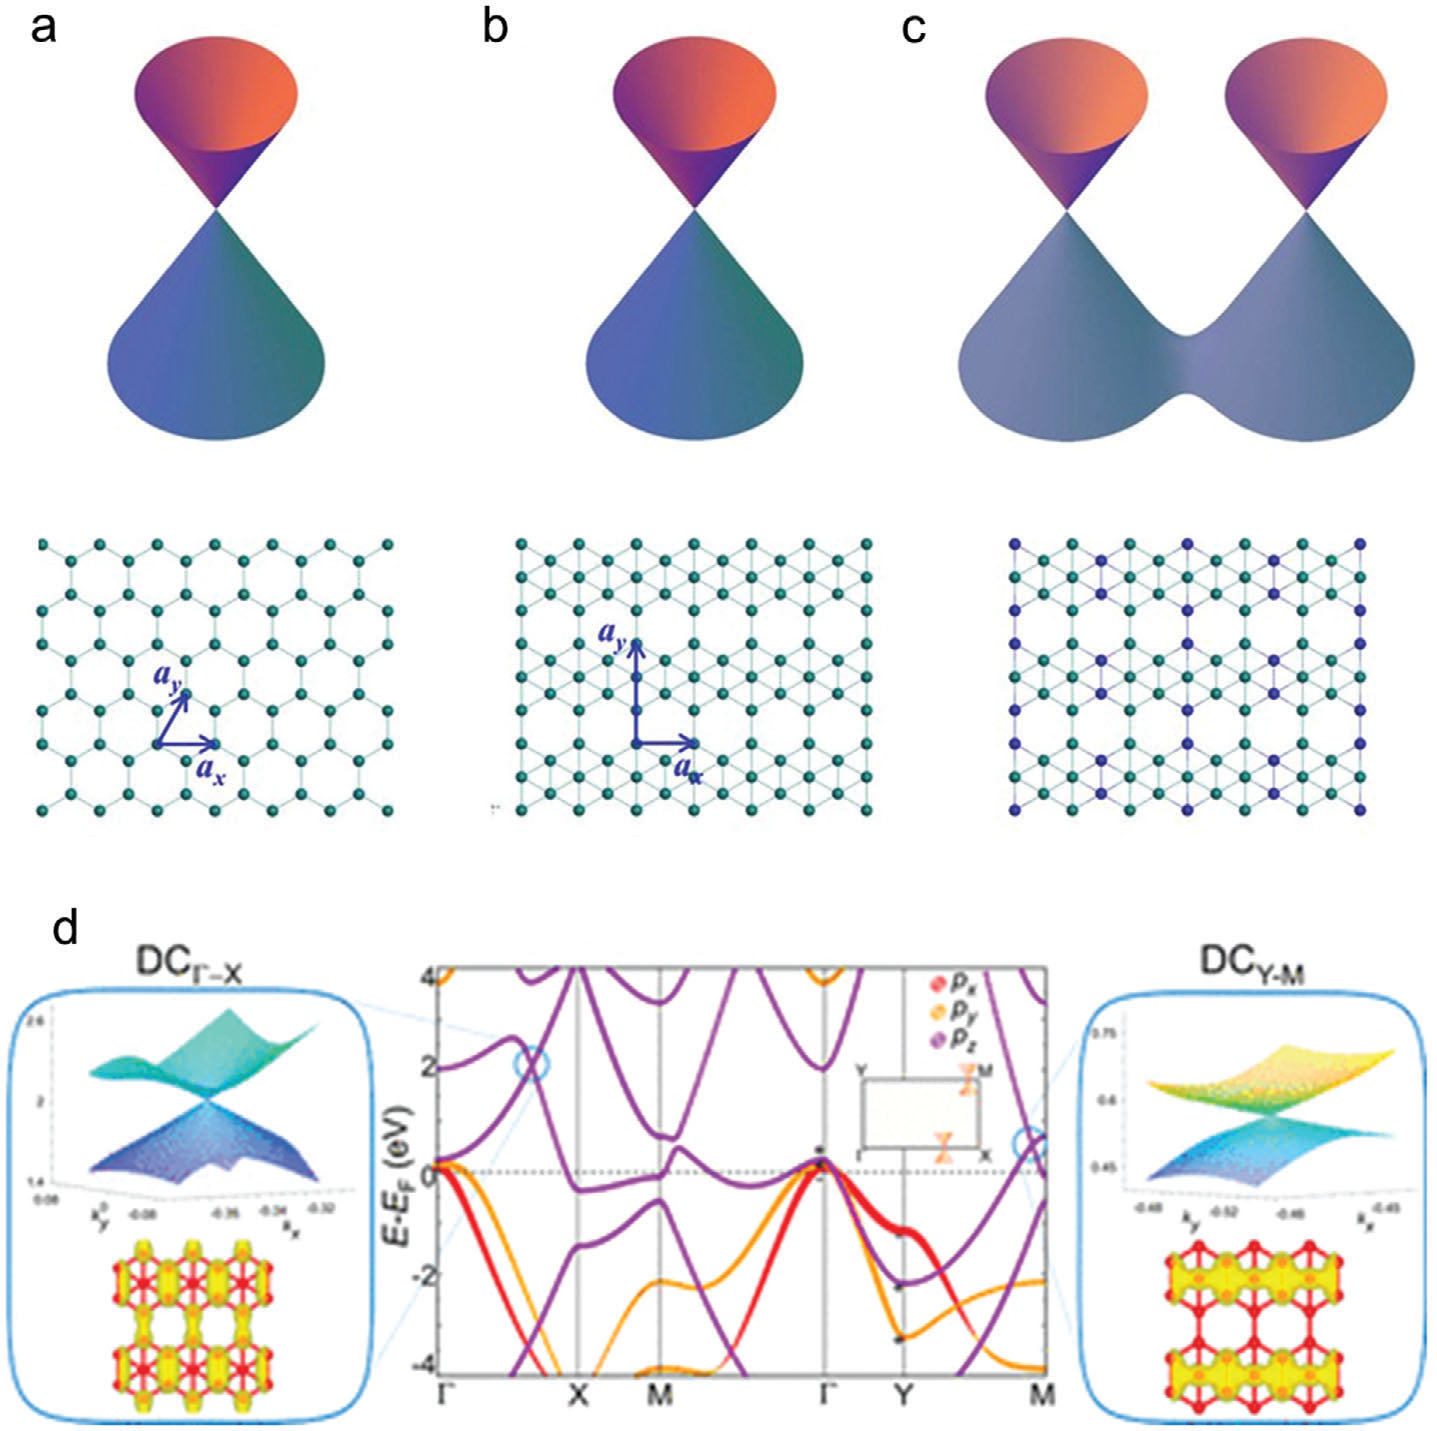
\includegraphics[width=\linewidth]{Diraccone.png}
    \caption{مخروط های دیراک و شبکه های الف) بوروفن لانه زنبوری. ب) بوروفن β12. ج) بوروفن β12 با اغتشاش 3×1. الف – ج) با اجازه استنساخ.[129] د) ساختار نواری بوروفن β12 (مرکز)، و نمای سه‌بعدی مخروط دیراک (DCΓ-X، سمت چپ) و مخروط دیراک (DCY-M، سمت راست) با نمودار چگالی ایزوشارژ تجزیه‌شده نواری}
    \label{fig:Diraccone}
\end{figure*}
ابتدا با محاسبات اولیه در سال 2017 تأیید شد که 12 بوروفن دارای فرمیون های دیراک است که به طور تجربی اولین ماده دیراک تک لایه غیر لانه زنبوری را تأیید کرد. گزارش شده است که نوارهای $\pi$ نزدیک سطح فرمی $\beta_{12}$ بوروفن از مدار $p_z$ مانند گرافن جدا شده است. علاوه بر این، تنها با در نظر گرفتن مدار pz روی بوروفن $\beta_{12}$ مستقل، مخروط های دیراک در $(±2\pi/3a، \theta)$ از اولین منطقه بریلوین \lr{(BZ)} در بوروفن 12 مستقل از طریق یک مدل اتصال محکم ساده آشکار شدند. مشابه شبکه لانه زنبوری، $\beta_{12}$ بوروفن را می توان به دو زیرشبکه مثلثی متلاشی کرد و در نتیجه مخروط دیراک میزبان، و شکافتن مخروط های دیراک تحت تأثیر تقارن زیرشبکه قرار می گیرد (شکل \ref{fig:Diraccone}\ref{}\lr{6a-c}). در همین حال، ماتسودا و همکاران. همچنین پیشنهاد کرد که هر مخروط دیراک را می توان با استفاده از اغتشاشات تناوبی تقسیم کرد و مخروط های شکافته دیراک غیر متمرکز هستند و با گرافن متفاوت هستند. گوپتا و همکاران.[136] منشا فرمیونهای دیراک را به ترتیب در $\beta_{12}$ روی \lr{Ag(111)} و 12 بروفن مستقل کاوش کرده اند. بر اساس گزارش آنها، یک خط گره دیراک از نظر توپولوژیکی و دو مخروط دیراک در $\beta_{12}$ بوروفن وجود دارد که در میان آنها دو مخروط دیراک به ترتیب در امتداد جهت‌های $Gamma-X$(\lr{DCΓ-X}) و \lr{Y-M} (\lr{DCY-M}) قرار دارند. شکل \ref{fig:Diraccone}\lr{6d}). بعلاوه، اگرچه مخروط های دیراک بوروفن $\beta_{12}$ با پشتیبانی \lr{Ag(111)} می توانند شکاف ایجاد کنند. خط گره هنوز از نظر توپولوژیکی محافظت می شود. حالت‌های توپولوژیکی بی‌اهمیت در این 12 بوروفن می‌توانند از درک بیشتر خواص توپولوژیکی بوروفن حمایت کنند، و بنابراین به نفع ایفای نقش در تحقیقات و کاربردهای پایه هستند. در سال 2017، چن و همکاران.\cite{zhangDiracNodalLines2017}[137] یک ساختار بور 2 بعدی جدید به نام \lr{hr-sB} با دو نوع فرمیون دیراک مربوط به خط گره دیراک و مخروط های دیراک گرادیان ناهمسانگرد قوی جدا از هم، متفاوت از مخروط های دیراک سنتی مشاهده شده در $\beta_{12}$ پیش بینی کرد. با الهام از ساختار لانه زنبوری در گرافن، تحقیقات مربوط به مخروط‌های دیراک بور درون صفحه‌ای لانه زنبوری نیز جذاب است. علاوه بر این، یک اکسید بوروفن لانه زنبوری به نام \lr{h-B2O} که اخیراً یافت شده است، دارای رسانایی عالی به عنوان فلز حلقه گره‌ای توپولوژیکی دوبعدی است و بنابراین یک ماده آند بسیار امیدوارکننده برای باتری‌هایی با ظرفیت بسیار زیاد است.\cite{hu2DHoneycombBorophene2020}[138] امروزه مطالعات مربوط به خواص توپولوژیکی به مدل فرمیون های ویل یا دیراک محدود نمی شود و تجزیه و تحلیل تقارن به کریستال های دارای نظم مغناطیسی و برهمکنش‌ها نیز کشیده شده است.\cite{bradlynDiracWeylFermions2016}[139] اخیراً \lr{Ezawa} و همکاران.\cite{ezawaTripletFermionsDirac2017}[140] پیشنهاد کرد که ممکن است فرمیون های سه گانه در 12 بروفن وجود داشته باشد و تئوری های سه باندی برای فرمیون های سه گانه ساخت. همه درک بالا از خواص توپولوژیکی مواد بور دوبعدی، پایه محکمی را برای تحقیقات بعدی کاربرد الکتریکی ایجاد می کند.\cite{fanCatScradlelikeDirac2018}[141]
\subsection{ابررسانایی}
گزارش شده است که جرم اتمی نسبتاً کم بور می تواند جفت الکترون-فونون قوی ایجاد کند، و فلزی بودن بوروفن می تواند باعث ایجاد غلظت حامل بالاتری شود، \cite{kortusSuperconductivityMetallicBoron2001, choiOriginAnomalousSuperconducting2002, anSuperconductivityMgB2Covalent2001}[142-144] که هر دو از عوامل کلیدی در تشکیل ابررساناهای معمولی هستند. ، ثابت می کند که بوروفن پتانسیل تبدیل شدن به یک ابررسانا را دارد. شایان ذکر است، یاکوبسون و همکاران.\cite{penevCanTwoDimensionalBoron2016}[120] دمای بحرانی آن را $T_c$ نسبت به گرافن پیش بینی کرد ($T_c ≈ 8.1\; K$ در تئوری \cite{profetaPhononmediatedSuperconductivityGraphene2012}[145] و \lr{4.5 K} از نظر تجربی).\cite{xueSuperconductivityPotassiumDopedFewLayer2012}[146] با این وجود، دوپینگ الکترون و کرنش کششی می‌توانند باعث سرکوب ابررسانایی برای بوروفن شوند، \cite{chengSuppressedSuperconductivitySubstratesupported2017, xiaoEnhancedSuperconductivityStrain2016}\cite{wuLithiumBoronLiBMonolayers2016}[147-149] که تشخیص دمای بحرانی بوروفن در آزمایش‌ها را دشوار می‌سازد. با این حال، هنگامی که به این مسائل پرداخته شد، این ویژگی ها انعطاف پذیری طراحی و راحتی برای بوروفن را در دستگاه های ابررسانا افزایش می دهد.
\section{نیمه رسانایی}
دانشمندان به طور تجربی نشان داده‌اند که چندین فاز بوروفن به دلیل وجود شکاف‌های باند غیرصفر دارای نیمه‌رسانایی هستند. دریافتند که صفحات $\alpha-$و $\alpha\prime-$ (ورق کمی کمانش شده) هر دو نیمه هادی های با شکاف کوچک با فاصله باند غیرمستقیم 1.40 و \lr{1.10 eV} هستند که در میان آنها ورق $\alpha\prime$ بیشترین انرژی منسجم را دارد و احتمالاً بیشترین انرژی منسجم را دارد. بوروفن کماندار پایدار کو و همکاران.\cite{kouHighmobilityAnisotropicTransport2016}[151] دریافتند که اگرچه حداقل است، اما باز هم می توان با تغییر تنش اعمال شده، شکاف باند سطح بوروفن ضخیم تر را تغییر داد، که باعث تغییر بیشتر در تحرک الکترون و در نتیجه تبدیل نوع رسانایی بوروفن از فلزی به نیمه هادی می شود. در این حالت، تحرک الکترون بالاتری را می توان با تغییر تنش اعمال شده به دست آورد. بنابراین، $\gamma-B_28$ بوروفن دارای چشم انداز کاربردی در زمینه دستگاه های حساس به فشار و حساس به نور است.

\subsection{حالت های الکترونی تقریباً آزاد 1 بعدی}
\cite{eknapakulNearlyfreeelectronSystemMonolayer2016, fengElectronicPropertiesSuperatom2011}[152،153] حالت‌های تقریباً الکترون آزاد \lr{(NFE)} که با جرم مؤثر تقریباً مطابق با جرم الکترون آزاد ($m_e$) مشخص می‌شوند، پراکندگی انرژی سهموی را نشان می‌دهند، که خواص انتقال الکترون آن نسبتاً قابل‌توجه است و می‌تواند در گسیل‌کننده‌های الکترون اعمال شود.[154،155]. حالت‌های \lr{NFE} می‌توانند به طور گسترده روی سطوح مواد با ابعاد کم که پتانسیل محصور شدن به آنها عمود است وجود داشته باشند، مانند مولکول‌های \lr{$\theta_D$ \ch{C60}}، \cite{zhaoSuperatomStatesFullerenes2009, fengAtomlikeHollowcoreboundMolecular2008}[156،157] نانولوله‌ها و نانوروبان‌های 1 بعدی، \cite{yamanakaElectronInjectionNearly2014, huNearlyFreeElectron2010}[158،159] و گرافن 2 بعدی، \cite{silkinImagePotentialStates2009}[160] در حالی که به دلیل وجود شیب پتانسیل معمولاً به صفحه پایه مواد نرمال است، این حالت های \lr{NFE} ترجیح می دهند به جای ماندن در اطراف صفحه پایه، در ناحیه خلاء گسترش یابند، بنابراین محدودیت هایی را بر برتری آنها در خواص انتقال اعمال می کنند.\cite{kongOnedimensionalNearlyFree2019}[161] وو و همکاران \cite{kongOnedimensionalNearlyFree2019}[161] حالت‌های \lr{NFE} 1 بعدی غیرمحلی را در یک اتصال همو بوروفن با پشتیبانی \lr{Ag (111)} مشاهده کرده‌اند که از دو (2،3) دامنه (یعنی صفحه v1/6 \cite{zhangTwoDimensionalBoronMonolayers2015}[162] یا $\beta_{12}$ \cite{fengExperimentalRealizationTwodimensional2016}[13]) تشکیل شده است که این دو را به هم متصل می‌کند (2، 2) نوارها به عنوان یک نقص خط، با استفاده از \lr{STM} همراه با محاسبات اصول اول. قابل توجه است که حالت های \lr{NFE} در بوروفن با سایر مواد کم بعدی که در بالا ذکر شد کاملاً متفاوت است. که اولی هنوز در نزدیکی سطح بوروفن به دلیل شیب پتانسیل درون صفحه ای شکل گرفته است و اختلال کمتری در امتداد عمود بر صفحه را تجربه می کند. این مکانیسم منحصر به فرد به این معنی است که حالت های \lr{NFE} موجود در بوروفن ممکن است در زمینه انتقال بار اعمال شود. با هدف این کشف مهم، وو و همکاران. تلاش کرد تا با تعمیق چاه پتانسیل، حالت \lr{NFE} را نزدیک تر به سطح فرمی تغییر دهد تا این حالت بتواند انتقال الکترون را بسیار بهتر تحت تأثیر قرار دهد. در نهایت، محاسبات جامع نشان می‌دهد که موقعیت بهینه برای حالت \lr{NFE} کمی فراتر از سطح فرمی قرار می‌گیرد، به طوری که با اعمال کرنش درون صفحه‌ای 2\% عمودی به نقص خط و در نتیجه القای انتقال الکترون به طور موثر در انتقال الکترون شرکت می‌کند. چاه بالقوه عمیق تر علاوه بر این، حالت‌های \lr{NFE} ممکن است یک کانال انتقال بالستیک ایده‌آل را به دلیل عدم حساسیت آن به پراکندگی حمل و نقل فراهم کنند، که می‌تواند به دستیابی به زمان آرامش حمل و نقل بسیار طولانی‌تر برای کاهش تولید گرما و مقاومت الکترون کمک کند.
\section{خواص حرارتی}
بوروفن دارای خواص حرارتی استثنایی از جمله پایداری حرارتی و هدایت حرارتی است. در سال های اخیر مطالعات نشان داده است که خواص حرارتی آن رابطه زیادی با ساختار بوروفن دارد. پایداری حرارتی و هدایت حرارتی بوروفن به تفصیل در زیر توضیح داده خواهد شد. در سال‌های اخیر، بسیاری از انواع مختلف بوروفن از نظر تئوری پیش‌بینی و تأیید تجربی شده‌اند، \cite{fengExperimentalRealizationTwodimensional2016, mannixSynthesisBorophenesAnisotropic2015, wuTwoDimensionalBoronMonolayer2012}[13،36،43] از جمله فازهای 12، $\delta_6$ و $\chi_3$ که به صورت همبستگی روی \lr{Ag(111)} رشد کردند. پس از جدا شدن از بستر، ممکن است از نظر حرارتی ناپایدار باشند، به خصوص در فاز $\delta_6$. برای کنترل ناپایداری $\delta_6$ فاز بوروفن، ژو و همکاران.\cite{zhouMolecularDynamicsSimulations2017}[106] دو پتانسیل تجربی کارآمد را برای شبیه‌سازی دینامیک مولکولی ایجاد کرد تا تعامل بین ساختارهای مثلثی کم انرژی و بوروفن را نشان دهد: حالت میدان نیروی ظرفیت بالقوه خطی و پتانسیل غیرخطی استیلینگر-وبر. علاوه بر این، استراتژی دیگر برای از بین بردن ناپایداری بوروفن، تولید بوروفن کاملاً هیدروژنه شده است. جالب توجه است که مطالعات اخیر نشان داده است که بوروفن خواص ویژه ای در حمل و نقل حرارتی از خود نشان می دهد که با توجه به ساختار آن متفاوت است. به طور کلی، هنگامی که هادی در یک گرادیان دما قرار دارد، انتقال حرارتی شار حرارتی است، در حالی که این فرآیند دارای یک مکانیسم انتقال فونون و پراکندگی پیچیده است.[134] با استفاده از تابع گرین غیرتعادلی \lr{(NEGF)} و محاسبات اولیه، \cite{zhouSuperiorLatticeThermal2017}[29] مشخص شد که بوروفن رسانایی حرارتی شبکه ای برتری را در رژیم بالستیک نشان می دهد، که بیشتر از گرافن است. این می تواند ناشی از جرم نور، پیوندهای کوتاه \lr{B-B}، انتقال فونون غیر معمول، ناهمسانگردی ساختاری قوی بوروفن باشد که منجر به سرعت گروه فونونی بالاتر می شود. به طور کلی، زمانی که طول نمونه کوتاهتر از مسیر آزاد میانگین فونونی مجاز آن باشد.\cite{mortazaviAnomalousStrainEffect2017}[166] هدایت حرارتی محاسبه شده توسط \lr{MD} با افزایش طول نمونه افزایش می‌یابد، که شبیه معادله انتقال فونون بولتزمن است. که پراکندگی فونون خارج از صفحه را افزایش می دهد و منجر به انتقال حرارتی انتشار قوی تر می شود.\cite{liuRecentProgressGrapheneanalogous2019}[110] علاوه بر این، ساختار حجیم در بوروفن، انتقال حرارتی آن را ناهمسانگرد می کند. فرکانس فونون فازهای مختلف بوروفن به هم نزدیک است زیرا بوروفن از یک اتم بور تشکیل شده است. با این وجود، مقادیر اتم‌های بور در هر سلول واحد یکسان نیست، که منجر به تقارن‌های هندسی متمایز و تعداد متفاوتی از شاخه‌های فونون نوری می‌شود که منجر به انتقال حرارتی متعدد می‌شود. در بوروفن تقریباً همسانگرد است، در حالی که برای فونون های فرکانس بالا، انتقال یک بعدی است که منجر به هدایت حرارتی فوق العاده بالا می شود. \cite{zhouSuperiorLatticeThermal2017}[29] این نشان می دهد که نرخ های مختلف پراکندگی فونون منجر به تفاوت های مشاهده شده در هدایت حرارتی و خواص حرارتی می شود. به عنوان مثال، 12 فاز بوروفن بسیار ناهمسانگرد است در حالی که فاز 12 همسانگرد است. فاز $\alpha$ ذاتاً پایدار است، در حالی که فاز 6 از نظر حرارتی ناپایدار است. \cite{zhouSuperiorLatticeThermal2017, xiaoLatticeThermalConductivity2017}\cite{tsafackThermomechanicalAnalysisTwodimensional2016}[29،30،165] خواص حرارتی ویژه بوروفن که در بالا توضیح داده شد، راهنمایی برای کاربرد احتمالی این مواد، قادر به برآوردن نیازهای مختلف صنایع مختلف است. به عنوان مثال، رسانایی حرارتی بالا می تواند به حذف گرمای انباشته در تجهیزات فتوولتائیک و الکترونیکی کمک کند، در حالی که صنایع ترموالکتریک و عایق حرارتی به مواد رسانایی حرارتی کم نیاز دارند. تعدد حمل و نقل حرارتی در بوروفن، کاربرد آن را در مدیریت حرارتی و رساناهای شفاف ممکن می سازد.
\section{کاربردهای بوروفن}
مقدار زیادی از داده‌های نظری و تجربی نشان داد که بوروفن دارای خواص عالی با پتانسیل در کاربردهای مختلف در زمینه‌های بسیاری مانند ذخیره‌سازی انرژی، \cite{raoUltrahighEnergyStorage2017}[168] دستگاه‌های الکترونیکی، \cite{pengTuningElectronicStructure2016, mortazaviBoropheneAnodeMaterial2016}[169-171] و زیست‌پزشکی، \cite{jiNovelTopDownSynthesis2018}[25] از جمله موارد دیگر است. اندازه و خواص فیزیکوشیمیایی بوروفن نقش تعیین کننده ای در کاربرد بیشتر آن در دستگاه های الکترونیکی و بسیاری از زمینه های دیگر دارد. با این حال، تولید در مقیاس بزرگ بوروفن سطح بزرگ در آزمایشگاه همچنان چالش برانگیز است. بوروفن تولید شده در حال حاضر از نظر اندازه کوچک (سطح نانومتری) و در حالت آزاد ناپایدار است، که نشان دهنده موانعی برای کاربرد بیشتر بوروفن در دستگاه های الکترونیکی است، اما در زیست پزشکی قدرت نشان می دهد. مواد با اندازه نانو در زمینه درمان تومور محبوب هستند. از آنجایی که اثر نفوذپذیری و احتباس \lr{(EPR)} افزایش یافته تومورها، حامل‌های دارو با اندازه‌های بین 10 تا 1000 نانومتر در محل تومور غنی‌سازی می‌شوند تا هدف‌گیری غیرفعال تومورها و بهبود اثربخشی داروها و کاهش جانبی انجام شود. اثرات. تحویل هوشمند داروها اغلب نیاز به اصلاح گروه‌های خاص بر روی حامل برای دستیابی به رهاسازی دقیق در محل تومور یا افزایش پایداری سیستم تحویل در بدن دارد. حامل مواد مخدر بور با توابع ویژه، بلکه چالش های ثبات بور را نیز حل می کند. در اینجا، ما کاربردهای اخیر بوروفن را بررسی می کنیم که عمدتاً بر زمینه های نوظهور زیست پزشکی تمرکز دارد.
\subsection{ابرخازنها}
ابرخازن نوع جدیدی از دستگاه ذخیره‌سازی انرژی است که دارای ویژگی‌های قابل توجه هزینه کم، عمر چرخه طولانی، سرعت شارژ/دشارژ سریع، چگالی توان بالا و چگالی انرژی کم است. بر اساس مکانیسم ذخیره بار سطحی، رسانایی الکتریکی و مساحت سطح مواد الکترود به‌طور برجسته‌ای بر عملکرد ابرخازن تأثیر می‌گذارد. با تحرک الکتریکی فوق العاده بالا، سطح بسیار زیاد، و ضخامت بسیار نازک.\cite{zhangBoropheneExtremelyHigh2016, zhanBoronSupercapacitors2016}[184,185] تحقیقات نظری اخیر نشان داده است که بوروفن، به عنوان یک ماده دو بعدی، خواص بهتری نسبت به گرافن در برخی جنبه های الکتروشیمیایی از خود نشان می دهد، بنابراین یک ماده الکترود امیدوارتر برای باتری‌ها و باتری‌ها است. ابرخازنها. این خصوصیات به شرح زیر است: 
\begin{figure*}
    \centering
    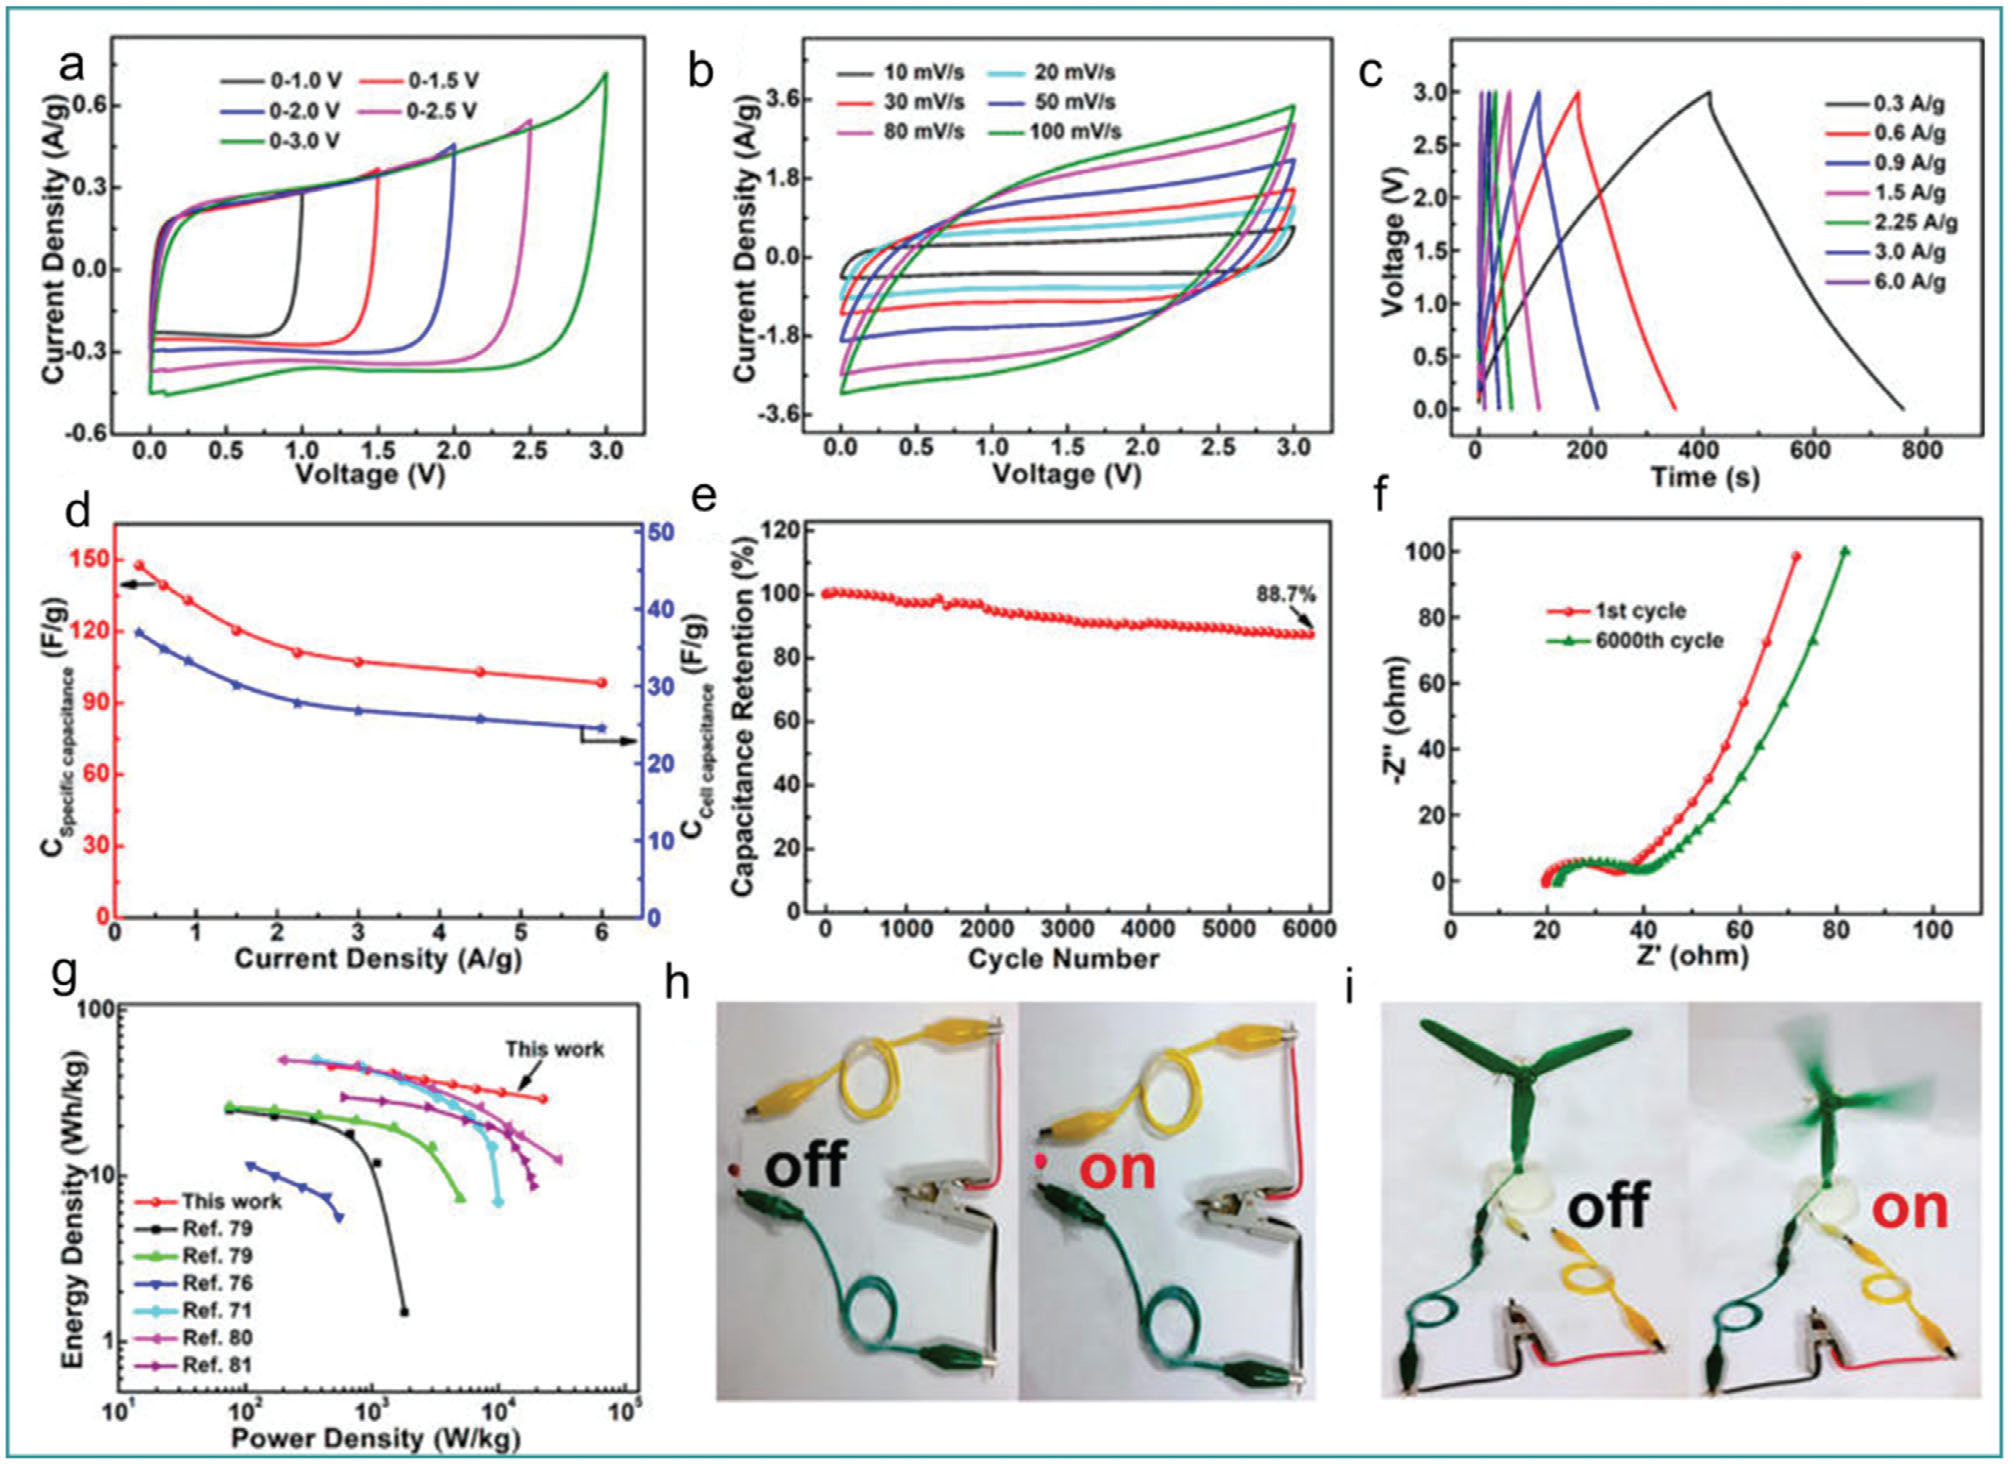
\includegraphics[width=\linewidth]{electricalproperties.png}
    \caption{خواص الکتروشیمیایی ابرخازن مبتنی بر ورق B آماده شده الف) منحنی های ولتامتری چرخه ای که تحت ولتاژهای مختلف به دست می آیند. ب) منحنی های ولتامتری چرخه ای که تحت نرخ های مختلف اسکن جمع آوری شده اند. ج) منحنی های GCD تحت چگالی جریان های مختلف آزمایش شده اند. د) ظرفیت سلولی مربوطه (منحنی آبی) و ظرفیت خازنی ویژه (منحنی قرمز) تحت چگالی جریان های مختلف. ه) پایداری دوچرخه‌سواری برای 6000 سیکل (سرعت اسکن: 50 mV s-1). و) کرت های نایکیست در ابتدا و انتهای 6000 سیکل جمع آوری شد. ز) نمودار راگون در مایع یونی. باتری آماده شده می تواند به عنوان منبع تغذیه برای نور (h) و فن (i) استفاده شود. الف – من)}
    \label{fig:electricalproperties}
\end{figure*}
\lr{I}) پنجره ولتاژ بزرگ و پایدار: همانطور که در شکل \ref{fig:electricalproperties}\lr{7a} نشان داده شده است، ابرخازن مونتاژ شده با بوروفن لایه برداری شده با \lr{DMF} تا 3.0 ولت پنجره ولتاژ را نشان می دهد. علاوه بر این، شکل \ref{fig:electricalproperties}\lr{7b} نشان می دهد که حتی در سرعت اسکن \lr{100 $mV\; s^{-1}$}، تمام منحنی های ولتامتری حلقوی شکلی تقریبا مستطیلی را نشان می دهند، \cite{luHTiO2MnO2HTiO22013}[186] که نشان دهنده خاصیت شارژ/دشارژ سریع و رفتار خازنی نسبتاً خوبی است (شکل \ref{fig:electricalproperties}\lr{7c}) ). 

\lr{II}) ظرفیت ویژه خوب: در چگالی جریان 0.3 $A\; g^{-1}$، حداکثر ظرفیت ویژه \lr{147.6 $F\; g^{-1}$} به دست می آید (شکل \ref{fig:electricalproperties}\lr{7d}). حداکثر ظرفیت ویژه بسیار بالاتر از ابرخازن مبتنی بر مواد مبتنی بر کربن و بور فله است.[187\cite{liuElectrochemicalBehaviorGraphene2011, chenHighPerformanceSupercapacitors2011},188] 

\lr{III}) قابلیت سرعت عالی: چگالی جریان از 0.\lr{3-6.0 $A\; g^{-1}$}، حدود 20 برابر افزایش می یابد، [189,190] ظرفیت خازنی ویژه \lr{98.3 $F^{-1}$} است، و نرخ نگهداری ظرفیت \lr{66.6٪} است.\cite{liScalableProductionFewLayer2018}[86] 

\lr{IV})  پایداری چرخه خوب: شکل \ref{fig:electricalproperties}\lr{7e} نشان می دهد که حفظ ظرفیت ویژه اولیه هنوز \lr{88.7٪} پس از 6000 چرخه با سرعت اسکن \lr{50 $mV s^{-1}$} است، \cite{liScalableProductionFewLayer2018}[86] که برابر یا حتی بهتر از ابرخازن های مبتنی بر کربن است. ، حتی اگر پس از 6000 سیکل آزمایش شده توسط طیف سنجی امپدانس الکتروشیمیایی در شکل \ref{fig:electricalproperties}\lr{7f}، یک کاهش جزئی در ظرفیت وجود داشته باشد. 

\lr{V}) چگالی انرژی عالی: تحت چگالی توان \lr{478.5 $W kg^{-1}$}، چگالی انرژی \lr{46.1 $Wh\; kg^{-1}$} را می توان به دست آورد (شکل \ref{fig:electricalproperties}\lr{7g})،\cite{shaoHighperformanceFlexibleAsymmetric2013} [191] که برابر یا حتی بیشتر از ابرخازن های ساخته شده از کربن است. در کاربردهای عملی، پس از شارژ برای چند ثانیه، یک سلول سکه با موفقیت نور را روشن کرد (شکل \ref{fig:electricalproperties}\lr{7h}) یا فن را به حرکت درآورد (شکل \ref{fig:electricalproperties}\lr{7i}). بنابراین، با ویژگی‌های چگالی جرم کم، سطح ویژه بالا، رسانایی قابل‌توجه الکترونیکی و غیره، چشم‌انداز کاربرد نانومواد بوروفن برای فتوولتائیک‌های نسل بعدی و ذخیره انرژی بسیار امیدوارکننده است.

\section{باتری‌ها}
خواص فلزی بودن و وزن اتمی کم این امکان را فراهم می کند که بوروفن آند باتری‌ها باشد. مطالعات نظری نشان داده است \cite{atacaHydrogenStorageCalcium2009}[192] که وقتی جاهای خالی شش ضلعی توخالی ذاتی در بوروفن فلزات جذب شده مانند لیتیوم و سدیم را محکم نگه می دارد، پایداری کل سیستم بالا می ماند یا حتی بهبود می یابد. مهمتر از آن، بوروفن هیچ مشکل کلی از نظر انبساط حجمی جدی، سینتیک آهسته، و کاربرد کم بینابینی ندارد، که همگی در مواد آند رایج مانند \ch{NiCo2O4}، کربن سخت و \ch{Sn} وجود دارند.\cite{ponrouchHighCapacityHard2013, alcantaraNiCo2O4SpinelFirst2002, liuUltrasmallSnNanoparticles2015}[193-195] به طور خلاصه، بوروفن دارای است. مزایای زیر به عنوان آند، به ویژه برای باتری های لیتیوم و \lr{Na-Ion} همانطور که از نظر تئوری پیش بینی شده است.
\begin{figure*}
    \centering
    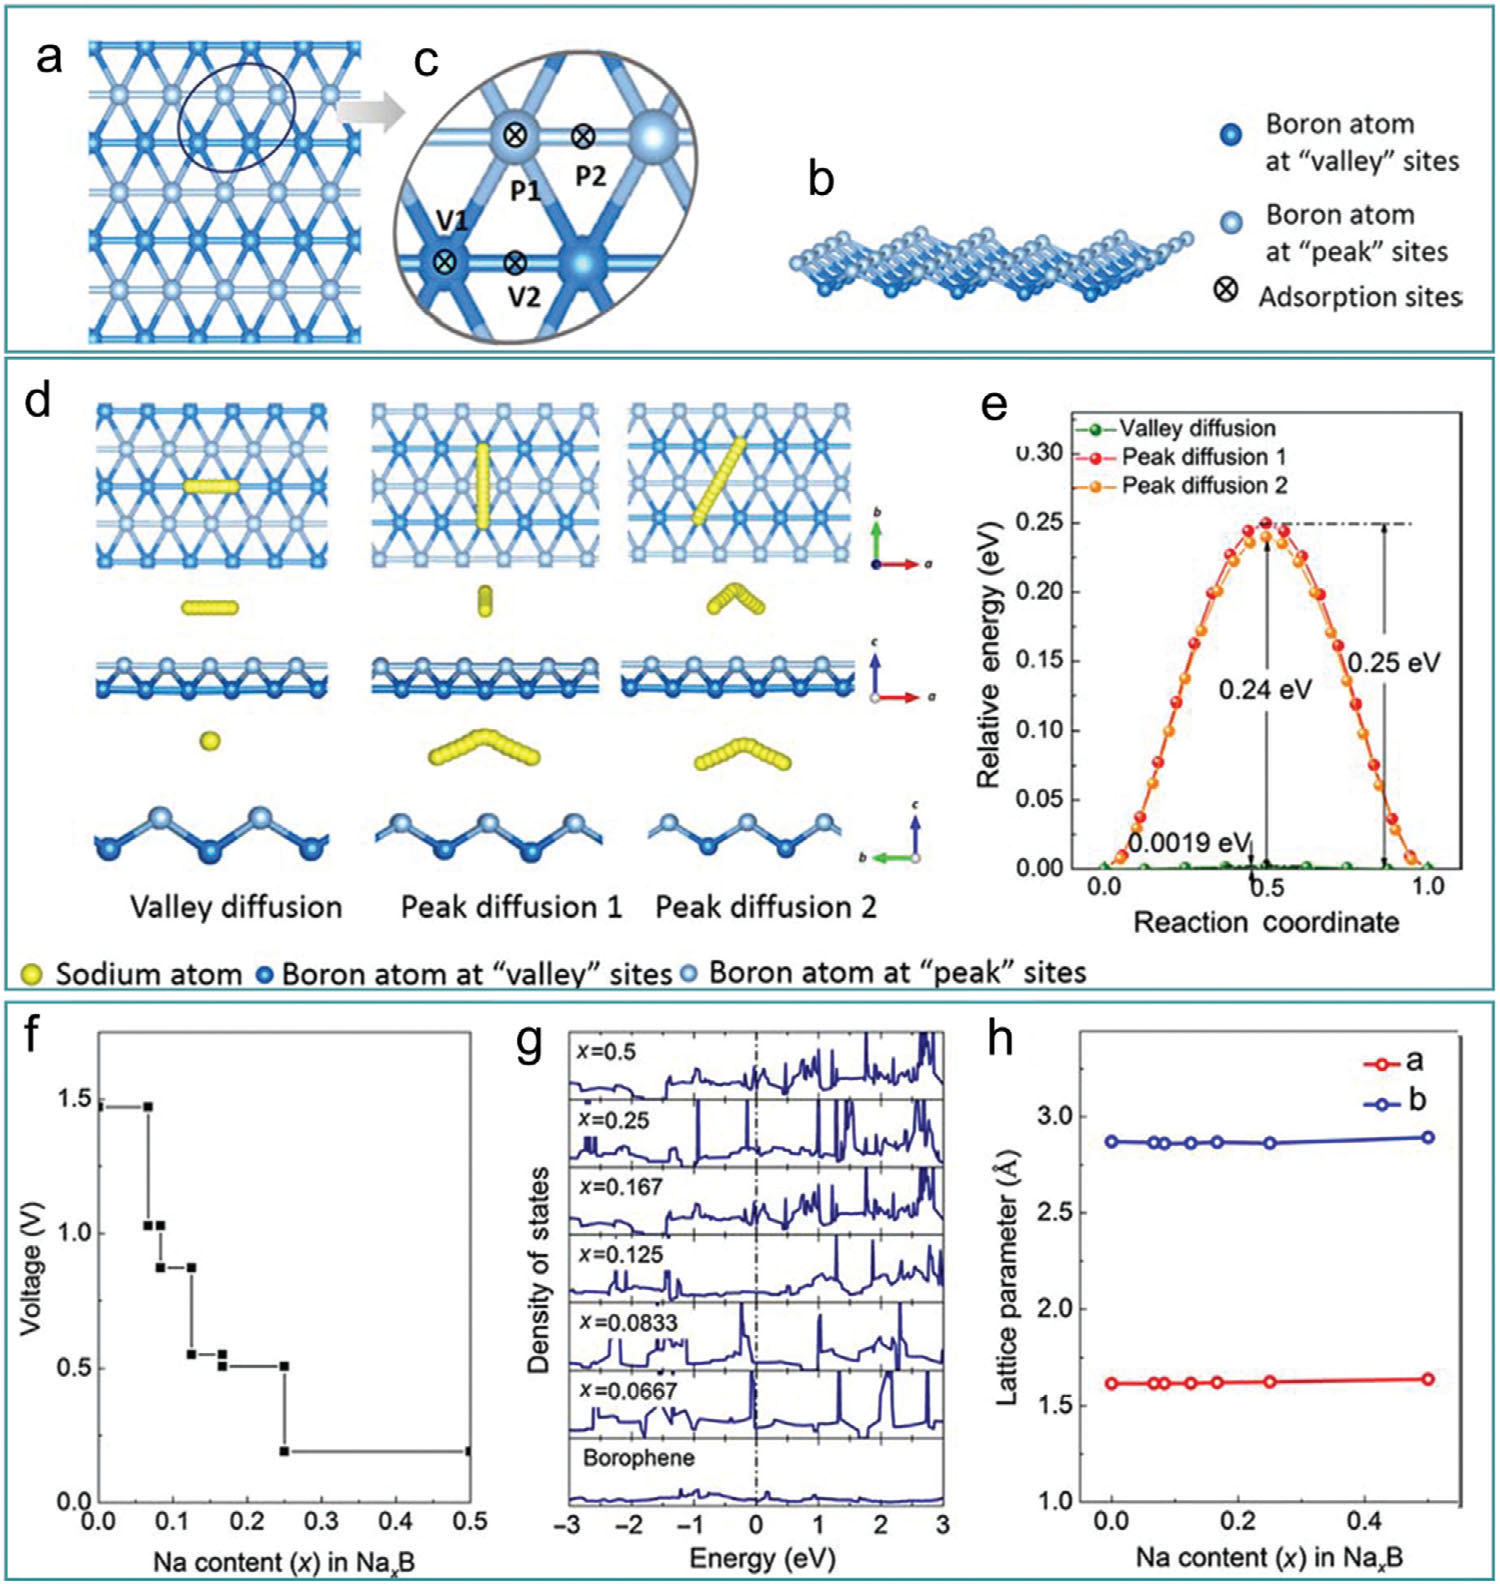
\includegraphics[width=\linewidth]{absorbtion.png}
    \caption{الف) نمای بالا، ب) نمای جانبی، و ج) محل های جذب انتخابی Pmmn بوروفن. د) سه مسیر انتشار سدیم روی بوروفن. ه) منحنی های انرژی مسیرهای انتشار. و) تغییر ولتاژ در طی فرآیند سدیاسیون. g،h) پارامترهای DOS و شبکه بوروفن تحت غلظت‌های مختلف سدیم. الف – ح) با اجازه تکثیر می شود.}
    \label{fig:absorbtion}
\end{figure*}
\subsection{خواص رسانا پایدار}
بوروفن \lr{Pmmn} ساختار کمانشی منحصر به فردی دارد (شکل \ref{fig:absorbtion}\lr{8a-c})، که در آن اتم‌های بور را می‌توان به دو گروه «قله» و «دره» با توجه به ارتفاع موقعیتشان تقسیم کرد.\cite{mannixSynthesisBorophenesAnisotropic2015}[36] ساختار لایه بسته بندی شل است، که می تواند پس از قرار گرفتن در غلظت های مختلف اتم های فلزی مانند سدیم و لیتیوم، انبساط حجمی کوچک (فقط \lr{2٪}) و تغییر شبکه را تضمین کند. بنابراین، بوروفن می تواند یکپارچگی ساختاری و پایداری چرخه خوبی را به عنوان ماده آند باتری نشان دهد.
\subsection{قابلیت نرخ فوق العاده}
بر اساس ساختار ویژه بوروفن، \lr{Xu} و همکاران.\cite{shiInitioPredictionBorophene2016}[196] با محاسبات \lr{DFT} یک سد انرژی انتشاری بسیار کم \lr{(0.0019 eV)} سدیم در "جهت دره" بدست آورد که بسیار کمتر از مواد آندی سنتی مانند \lr{Na2Ti3O7} و \lr{Na3Sb} (به ترتیب \lr{0.19} و \lr{0.21 eV}) است.[197,198] بیشتر. به طور شگفت انگیزی، نرخ انتشار در آن جهت بیش از 1000 برابر بیشتر از \lr{Na2Ti3O7} و \lr{Na3Sb} بود. \cite{baggettoIntrinsicThermodynamicKinetic2013, gonzeFirstprinciplesComputationMaterial2002, panSodiumStorageTransport2013}[197,199] در نهایت، سد انرژی انتشار \lr{Li} کمی بالاتر از سدیم از طریق خواص انتشار ناهمسانگرد بود (شکل \ref{fig:absorbtion}\lr{8d,e}). [171] همه این مشاهدات نشان می‌دهند که بوروفن توانایی نرخ قابل‌توجهی به عنوان آند باتری‌های لیتیوم یا \lr{Na-Ion}یون دارد، که به وضوح می‌تواند مشکل سینتیک کند را حل کند.\cite{shiInitioPredictionBorophene2016}[196]
\subsection{ظرفیت نظری فوق العاده بالا}
با در نظر گرفتن باتری های \lr{Na-ion} به عنوان مثال، زمانی که نسبت \lr{Na/B} (بوروفن) به 0.5 می رسد (سدیم به طور کاملاً یکنواخت دو طرف بالا و پایین بوروفن را می پوشاند)، مقدار ظرفیت نظری به حداکثر می رسد \lr{(1218 $mAh\; g^{-1}$)}. \lr{Na0.5B})، \cite{shiInitioPredictionBorophene2016}[196] که حداکثر مقدار و حدود سه برابر بیشتر از آند گرافیت \lr{(372 $mAh g^{-1}$)} است. وضعیت حتی برای لیتیوم \lr{(Li0.75B)} به دلیل شعاع اتمی بزرگتر، که ظرفیت نظری آن 1860 میلی آمپر ساعت در گرم 1 است، در حدود چهار برابر بیشتر از آند گرافیت است.\cite{jiangBorophenePromisingAnode2016}[171] بنابراین، بوروفن می‌تواند به طور قابل‌توجهی کاربرد میان‌افزایی فلزات را افزایش دهد، تراکم انرژی باتری و چگالی توان را افزایش دهد.

\subsection{جلوگیری موثر از تشکیل دندریت}
باتری‌های لیتیوم و \lr{Na-Ion} هر دو به دلیل داشتن فلزات بسیار واکنش‌پذیر با دمای ذوب پایین، با مسائل دندریت به چالش کشیده می‌شوند، \cite{mortazaviElasticSofteningAlloy2013, chevrierChallengesNaionNegative2011}[200,201] که یک نگرانی جدی ایمنی را نشان می‌دهد که هنوز به طور موثر حل نشده است. با این حال، بوروفن ممکن است بتواند این را معکوس کند. خو و همکاران \cite{shiInitioPredictionBorophene2016}[196] دریافت که میانگین ولتاژ مدار باز محاسبه‌شده یک باتری \lr{Na-ion} با بوروفن به عنوان ماده آند به اندازه 0.53 ولت در هنگام شارژ کردن است و پیوند بین بوروفن و \lr{Na} قوی است. (شکل \ref{fig:absorbtion}\lr{8f–h}). هر دو نشان می‌دهند که اتم‌های فلز به‌جای خوشه‌بندی برای تشکیل یک فاز فلزی جداگانه، به‌طور یکنواخت بروفن را پوشانده‌اند، که می‌تواند به طور مؤثری از تشکیل دندریت جلوگیری کند و در عین حال چگالی انرژی بالایی را حفظ کند. اگرچه داده‌های بالا نشان می‌دهند که بوروفن یک ماده آند باتری امیدوارکننده است، تحقیقات فعلی کاملاً تئوری باقی مانده است و آزمایش‌های وسیعی برای تأیید کاربردهای عملی آن هنوز مورد نیاز است.
\begin{figure*}
    \centering
    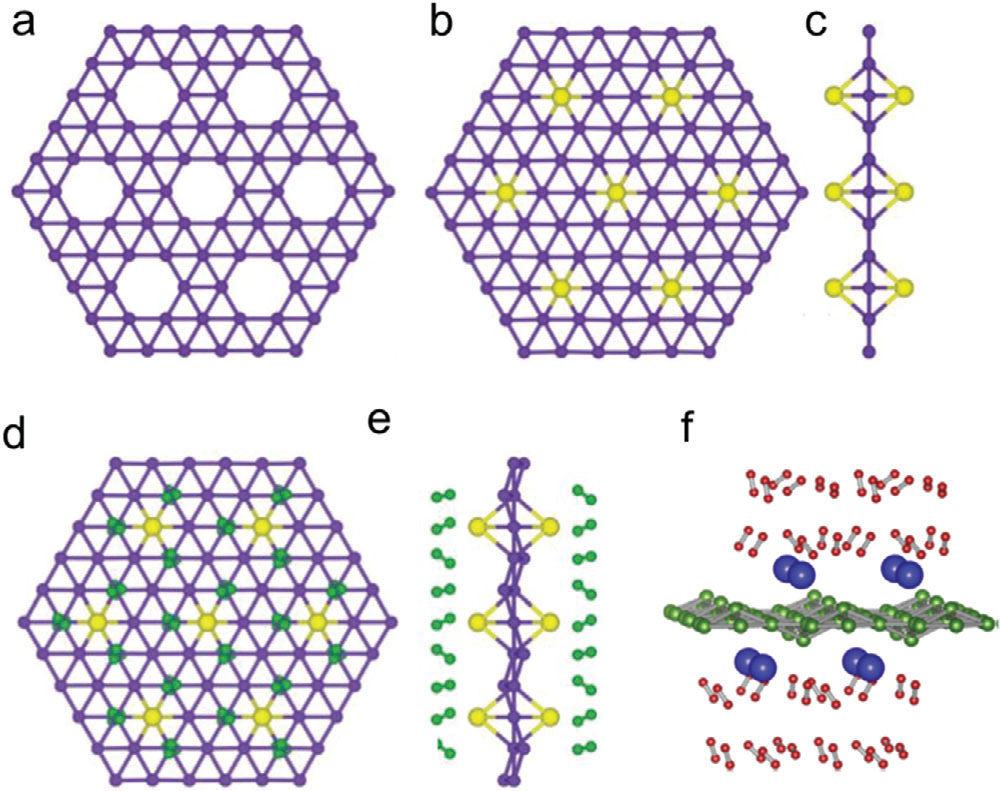
\includegraphics[width=\linewidth]{alphasheet.png}
    \caption{الف) ساختار بوروفن ورقه α بدون لیتیوم. ب، ج) ساختار بهینه شده بوروفن ورقه α با اتم های لیتیوم (کره های زرد). د، ه) ساختار بهینه شده بوروفن α-ورق با لیتیوم پس از جذب H2. الف-ه) ساختار بهینه‌شده بوروفن با تزئین کلسیم (کره‌های آبی) پس از جذب H2}
    \label{fig:alphasheet}
\end{figure*}
\section{ذخیره سازی هیدروژن}
با توجه به سوخت محدود و مسائل زیست محیطی، توسعه یک ماده مناسب برای ذخیره سازی هیدروژن ضروری است. برای ارزیابی توانایی ذخیره هیدروژن یک ماده، دو شاخص، یعنی انرژی جذب و ظرفیت جذب \ce{H2} مورد نیاز است. با توجه به انرژی جذب، انرژی جذب در محدوده \lr{0.2-0.6 eV} لازم است تا اطمینان حاصل شود که مولکول های \ce{H2} می توانند به طور پایدار و آسان روی سطح مواد جذب شوند. با توجه به ظرفیت جذب \ce{H2}، هدف تعیین شده توسط وزارت انرژی ایالات متحده 7.5 درصد وزنی است. اخیراً مشخص شده است که بوروفن به دلیل وزن سبک و مساحت سطح ویژه بزرگ، کاندیدای ذخیره‌سازی \ce{H2} است، به ویژه هنگامی که با گرافن یا فلزات واسطه اضافه می‌شود. از بوروفن خالص و دریافت که حداکثر کمتر از \lr{0.01 eV} است که برای ذخیره عملی \ce{H2} بسیار کوچک است. خوشبختانه، با کمک فلزات قلیایی یا واسطه، می توان فعالیت شیمیایی را افزایش داد و برهمکنش بین بوروفن و \lr{H2} را تقویت کرد. در طول جذب \ce{H2}، بوروفن نیازی به ایجاد نقص برای جذب فلزات ندارد، زیرا \lr{HH} های آن می توانند به عنوان مکان های جذب فلز استفاده شوند (شکل \ref{fig:alphasheet}\lr{9a-c}).\cite{shangTwoDimensionalBoron2018}[39] تانگ و همکاران \cite{tangTheoreticalInvestigationCalcium2018}[205] دریافت که $\beta_{12}$ فاز بوروفن با تزئینات کلسیم کاندیدای مناسبی برای ذخیره سازی \ch{2H} است. بوروفن فاز $\beta_{12}$ به طور طبیعی می تواند \lr{HH} ها را تشکیل دهد و به \ch{Ca} محل جذب خوبی می دهد (شکل \ref{fig:alphasheet}\lr{9f}).[206] ظرفیت جذب \ch{2H} حدود 8.92 درصد وزنی است. برای 3 فاز بوروفن با کلسیم؛ همچنین می‌تواند به ظرفیت جذب \lr{H2} 7.\lr{2 wt٪}، [202] نزدیک به گرافن دست یابد. برای مثال، بوروفن $\beta_{12}$ فاز دارای لیتیوم می تواند به ظرفیت جذب \lr{H2} 10.85 درصد وزنی دست یابد \cite{liuLiDecorated12BorophenePotential2017}[208] و ورقه تزئین شده با لیتیوم می تواند حداکثر 10.75 درصد وزنی \ch{2H} را جذب کند که نشان دهنده جذب حداکثر 3 مولکول \ch{2H} است. برای هر اتم لی (شکل \ref{fig:alphasheet}\lr{9d,e}).\cite{erDFTStudyPlanar2009}[209] علاوه بر این، بوروفن مثلثی کمانش شده با لیتیوم، ظرفیت جذب \ch{2H} 13.7 درصد وزنی است.\cite{shangTwoDimensionalBoron2018, liHighHydrogenStorage2017}[39,210] علاوه بر این، بوروفن تزئین شده با لیتیوم $(\nu= 1/8)$ با ظرفیت ذخیره سازی \ch{2H} 15.26 درصد گزارش شده است.\cite{liUltrahighCapacityMolecularHydrogen2015}[204] انرژی جذب و ظرفیت جذب \ch{2H} بوروفن تزئین شده با \ch{Ca/Li} در جدول 3 فهرست شده است. همه موارد فوق می توانند به اندازه کافی ثابت کنند که بوروفن با تزئینات \ch{Ca/Li} دارای پتانسیل آینده نگری در کاربردهای ذخیره سازی \lr{H2} است.
\begin{figure*}
    \centering
    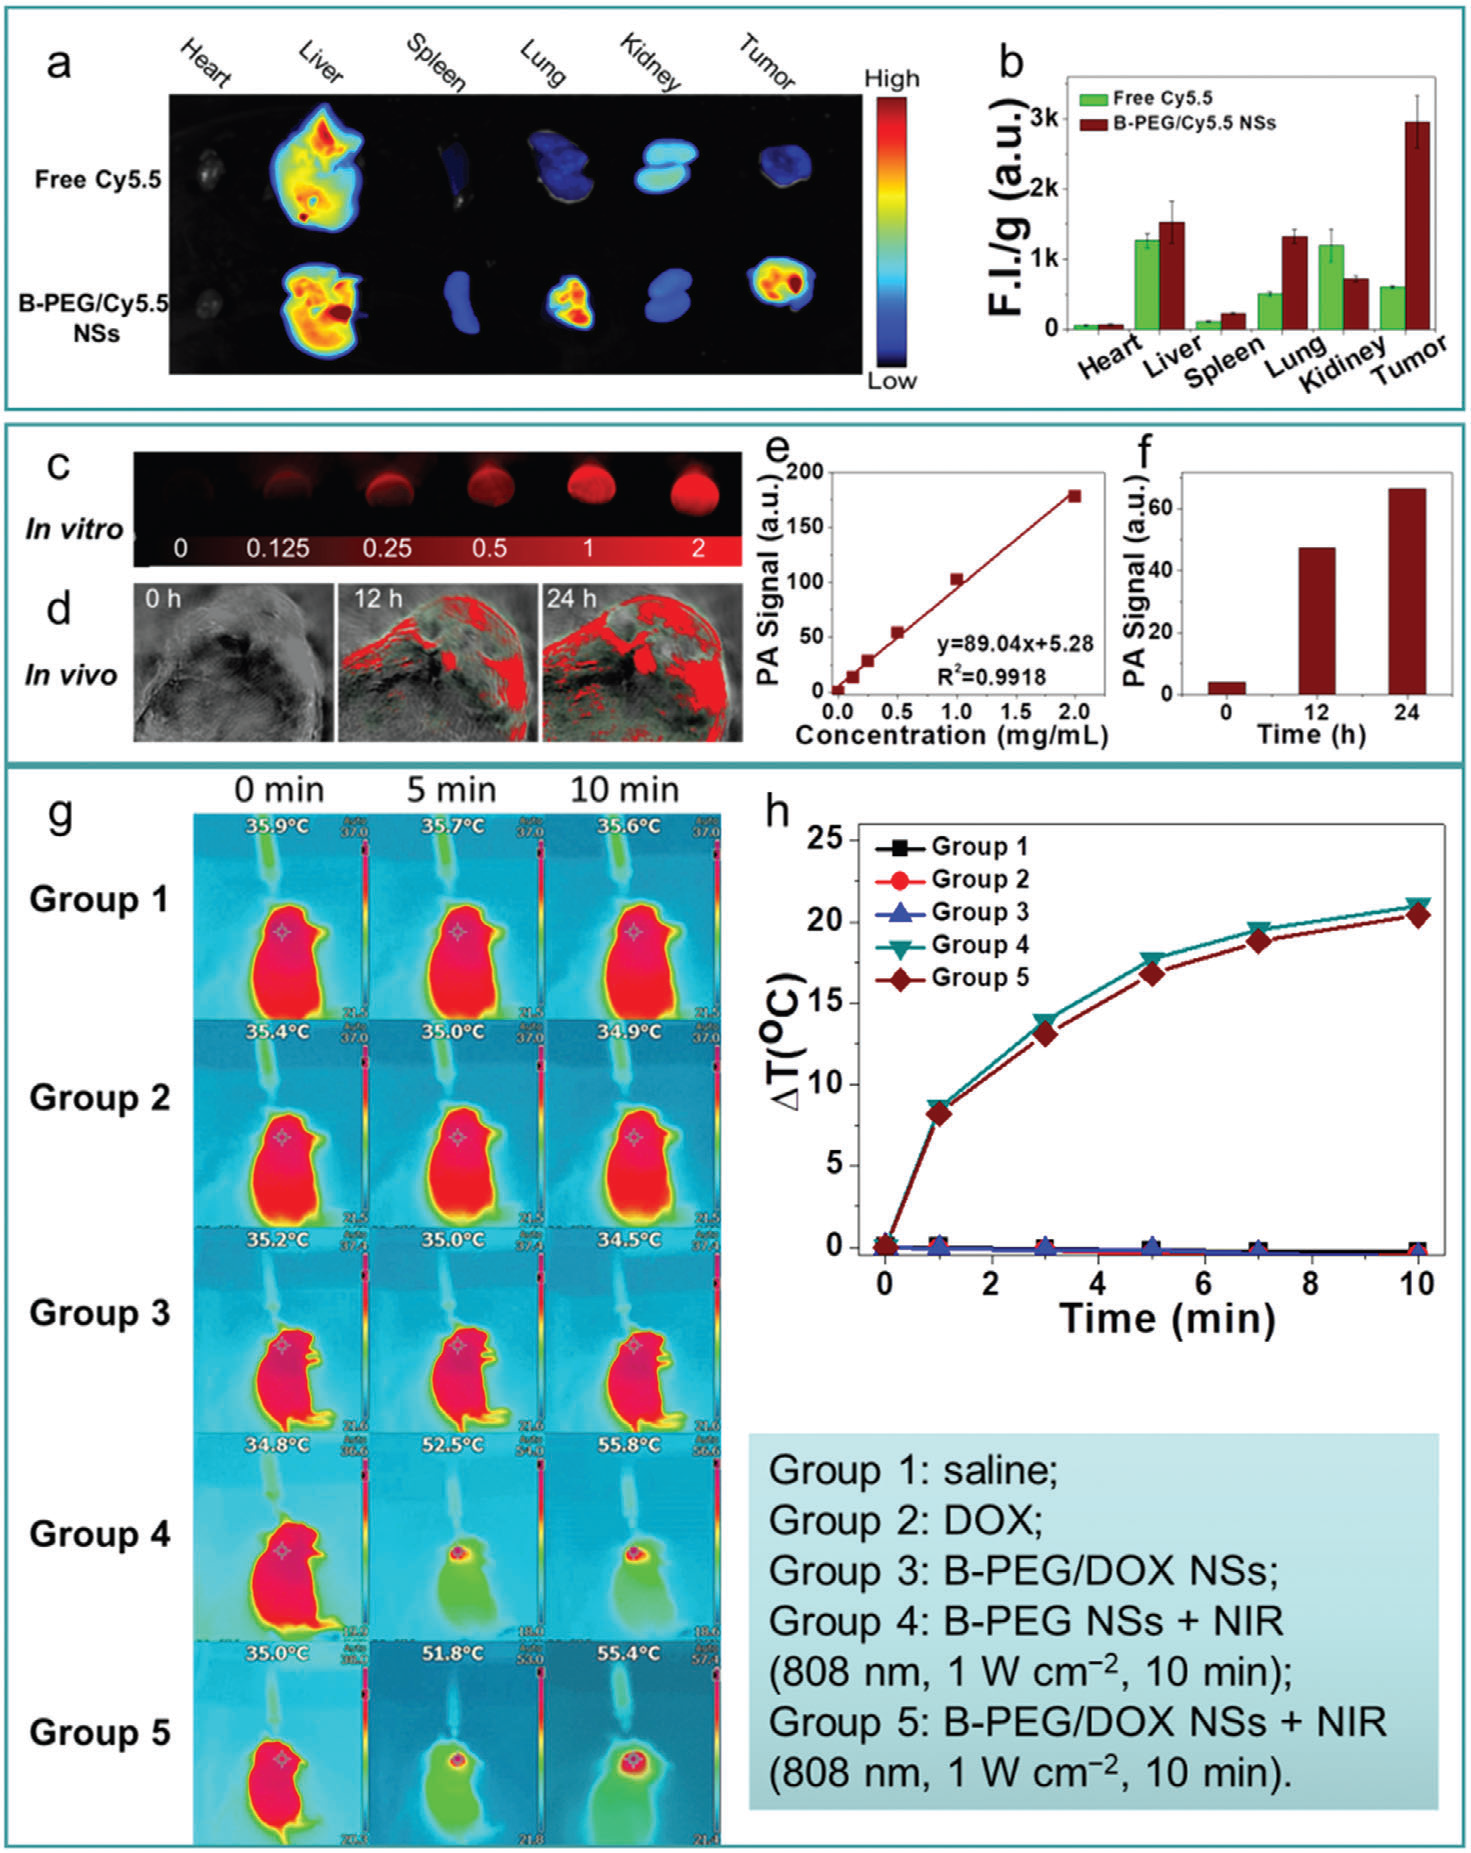
\includegraphics[width=\linewidth]{Multimodal.png}
    \caption{تصویربرداری چندوجهی از NS های مبتنی بر B. الف) تشخیص اندام ها و تومورهای اصلی با تصویربرداری فلورسانس. ب) توزیع زیستی نیمه کمی اندام های اصلی و تومورها. ج) تصاویر PA از B-PEG NSs با غلظت های مختلف (0، 0.125، 0.25، 0.5، 0.1، و 0.2 میلی گرم mL-1) در داخل بدن. د) تصاویر تومور PA. ه) رابطه خطی بین مقادیر PA و غلظت B-PEG NSs. و) تجزیه و تحلیل کمی مقادیر PA. ز) تصاویر فتوترمال و ح) مشخصات دمایی موش ها. a–h)}
    \label{fig:Multimodal}
\end{figure*}
\section{تصویربرداری زیستی}
تصویربرداری زیستی، از جمله تصویربرداری فلورسانس، \cite{gaoVivoCancerTargeting2004, medintzQuantumDotBioconjugates2005}[211،212] تصویربرداری فتوترمال، \cite{huangCancerCellImaging2006}[213] و تصویربرداری فوتوآکوستیک \lr{(PA)}، \cite{beardBiomedicalPhotoacousticImaging2011}[214] می‌تواند مکان و اندازه تومورها را فراهم کند و یک فناوری مهم برای تشخیص بالینی و درمان تومورها است. اطلاعات ضایعه نمایش داده شده توسط هر حالت تصویربرداری متفاوت است و هر حالت تصویربرداری مزایا و معایب خاص خود را دارد. بنابراین، اطلاعات تومور را می توان به طور جامع تری از طریق یک پلت فرم تصویربرداری چندوجهی تومور ارائه کرد، که می تواند تا حد زیادی خطر تشخیص اشتباه را کاهش دهد. جی و همکاران \cite{jiNovelTopDownSynthesis2018}[25] یک پلت فرم تصویربرداری چندوجهی تومور مبتنی بر بوروفن ساخته شد که می تواند به طور همزمان تصویربرداری فلورسانس، تصویربرداری \lr{PA} و تصویربرداری فتوترمال را انجام دهد. مواد فلورسنت بر روی حامل بارگذاری می شود و فرمولاسیون در تومور با روش های هدف گیری فعال یا هدف گیری غیرفعال غنی می شود. تصویر تصویربرداری فلورسانس از موش توموری که بوروفن نشاندار \ch{Cy5.5} اصلاح شده توسط \ch{PEG} (\lr{B-PEG} \ch{NS} با نشاندار \ch{Cy5.5}) تزریق شده است (شکل \ref{fig:Multimodal}\lr{10a,b}) به وضوح بین تومورهای بدخیم و بافت های طبیعی تمایز قائل شد. در مقایسه با رنگ فلورسنت رایگان \lr{Cy5.5}، \lr{B-PEG NS} با نشاندار \lr{Cy5.5} به دلیل اثر \lr{EPR}، زمان گردش خون طولانی‌تر و تجمع تومور بهتری دارد. علاوه بر این، \lr{B-PEG NS} نیز یک عامل بالقوه \lr{PA} است. تصویربرداری \lr{PA} یک روش تصویربرداری زیستی غیر مخرب است که از اولتراسوند به عنوان رسانه استفاده می کند. در مقایسه با تصویربرداری نوری و تصویربرداری صوتی، تصویربرداری \lr{PA} بر بسیاری از کاستی‌های این دو فناوری تصویربرداری غلبه کرده و عمق کاوش، کنتراست تصویر و وضوح فضایی را افزایش می‌دهد. تصویربرداری \lr{PA} می‌تواند نمودار ساختار تومور موش تومور را در زمان‌های مختلف پس از تزریق \lr{B-PEG NS} نشان دهد (شکل \ref{fig:Multimodal}\lr{10d,f})، و شدت سیگنال \lr{PA} با غلظت \lr{B-PEG NS} همبستگی مثبت دارد (شکل \ref{fig:Multimodal}\lr{10c}) ه) - هر چه غلظت \lr{B-PEG NS} بیشتر باشد، سیگنال قوی تر است. نتایج فوق نشان داد که \lr{B-PEG NS} می تواند به طور موثر در محل های تومور غنی شود و یک عامل بالقوه \lr{PA} است. علاوه بر این، بوروفن دارای نرخ تبدیل فتوترمال و پایداری فتوترمال خوبی است و انرژی نور را به انرژی گرمایی تحت تابش نور مادون قرمز نزدیک \lr{(NIR)} تبدیل می‌کند. توزیع بوروفن و تغییرات دما در اندام های مختلف را می توان با دوربین حرارتی مادون قرمز نیز بدست آورد. به عنوان مثال، در یک آزمایش، موش‌ها به پنج گروه تقسیم شدند، گروه‌های چهار و پنج پس از تزریق داخل وریدی \lr{B-PEG NSs} یا \lr{B-PEG/DOXNSs} (دوکسوروبیسین بارگذاری شده با \lr{B-PEG NSs}) و درجه حرارت در تومور این دو گروه از 308 به 328 کلوین افزایش یافت، در حالی که دمای سایر گروه‌ها بدون \lr{B-PEG NSs} یا \lr{NIR} در \lr{≈308K} ثابت ماند (شکل \ref{fig:Multimodal}\lr{10g,h}). در نتیجه، بوروفن را می توان به طور بالقوه در پلت فرم های تصویربرداری زیستی چندوجهی تومور مورد استفاده قرار داد و به دستیابی به تشخیص دقیق و درمان دقیق تومورها کمک کرد.
\begin{figure*}
    \centering
    \includegraphics[width=\linewidth]{UV.png}
    \caption{الف) طیف UV B-PEG NSs. ب) مشخصات تغییر دما B-PEG NSs تحت لیزر 808 نانومتر. ج) رابطه خطی بین -lnθ و زمان. د) مشخصات گرمایش B-PEG NSs پس از پنج سیکل. ه) اسکن تصاویر میکروسکوپ الکترونی عبوری–EDS از B-PEG/DOX NSs. و) طیف UV بارگیری بوروفن با DOX. ز) توانایی بوروفن برای بارگیری داروهای شیمی درمانی. ح) منحنی های DOX را تحت pH های مختلف آزاد کنید. i–n) آزمایشات سلولی. i) ارزیابی ایمنی بوروفن در سلول های مختلف (بدون لیزر). ی) ارزیابی سمیت بوروفن در سلول های مختلف (لیزر 808 نانومتر). ک) زنده ماندن نسبی سلول های تومور تحت درمان های مختلف. ل) تصاویر CLSM از سلول های تومور رنگ شده با PI (مرده، قرمز) و AM (زنده، سبز). م) عکسهای دیجیتالی موشها و تومورهای معرف در گروههای مختلف تحت درمان به مدت 14 روز. ن) وزن بدن موش ها. ج 1: کنترل؛ G2: داروهای شیمی درمانی. G 3: بوروفن + داروهای شیمی درمانی. G 4: بوروفن + لیزر 808 نانومتری. G 5: بوروفن + داروهای شیمی درمانی + لیزر 808 نانومتری. الف-ن)}
    \label{fig:UV}
\end{figure*}
\section{تحویل دارو }
انتشار موضعی داروهای شیمی درمانی کلید کاهش عوارض جانبی شیمی درمانی است. بنابراین، طراحی یک پلت فرم آزادسازی دارو با پاسخ ریزمحیط تومور هوشمند بسیار مهم است. سطح ویژه بسیار بالا بوروفن فضایی را برای بارگیری دارو و نقاط لنگر برای اصلاح گروه عملکردی فراهم می کند و آن را به ماده ای مناسب برای بسیاری از جنبه های درمان ضد سرطان تبدیل می کند. در یک سیستم دارورسانی مبتنی بر بوروفن، دوکسوروبیسین (DOX) با بوروفن انکوبه شد (نرخ بارگذاری: \lr{114\%}) و سیستم با \lr{PEG-NH2} پوشانده شد تا به گردش طولانی مدت داروهای شیمی درمانی در بدن دست یابد (شکل \ref{fig:UV}\lr{11e-g}). ) اصلاح موفقیت آمیز \lr{PEG} و بارگذاری \lr{DOX} را نشان داد.\cite{jiNovelTopDownSynthesis2018}[25] به عنوان یک حامل دارو، بوروفن \lr{pH} و واکنش گرمایی خوبی نشان داد. در \lr{pH 7.4} و \lr{pH 5.0}، نرخ آزادسازی \lr{DOX} توسط بوروفن به ترتیب \lr{8.3٪} و \lr{24٪} بود (شکل \ref{fig:UV}\lr{11h}). \lr{pH} ریزمحیط تومور کمتر از بافت طبیعی است (ادبیات)، که به بوروفن اجازه می دهد تا به رهاسازی هدفمند دارو در تومور دست یابد. علاوه بر این، بوروفن همچنین حامل دارو برای پاسخ \lr{NIR} است. تحت شرایط فوق، 5 دقیقه نور \lr{NIR} برای گروه‌های \lr{pH} مختلف اعمال شد، با سرعت انتشار دارو در \lr{pH 7.4} به \lr{41.4٪} و در \lr{pH 5.0} افزایش به \lr{77.6٪} (شکل \ref{fig:UV}\lr{11h}). به طور خلاصه، بوروفن با ظرفیت بارگیری دارو بالا و \lr{pH} و پاسخ دوگانه مادون قرمز، یک پلت فرم یکپارچه دارورسانی امیدوارکننده برای تشخیص و درمان سرطان است.\section{درمان سرطان}
نوردرمانی می تواند به درمان غیر تهاجمی/ کم تهاجمی سرطان دست یابد. این روش از تشعشعات \lr{NIR} برای تابش بافت تومور استفاده می کند و دمای بافت تومور به دلیل تبدیل فتوترمال افزایش می یابد و منجر به مرگ سلول های تومور می شود.\cite{prasadMechanismCellDeath2007}[215] یک عامل درمانی فتوترمال ایده آل باید سمیت کم، جذب نور قوی، راندمان تبدیل فتوترمال بالا و پایداری فتوترمال در پنجره \lr{NIR} (650-950 نانومتر) داشته باشد.\cite{jangGoldNanorodPhotosensitizerComplex2011, chengPEGylatedWS2Nanosheets2014}[216,217] \lr{Ji et al.}\cite{jiNovelTopDownSynthesis2018}[25] از بوروفن در درمان فتوترمال تومورها استفاده کرد و به اثرات درمانی خوبی دست یافت. سه معیار مهم برای یک عامل فتوترمال عالی عبارتند از: راندمان تبدیل فتوترمال، پایداری فتوترمال و جذب \lr{UV}. این خواص بوروفن مورد ارزیابی قرار گرفت. جذب \lr{UV-vis-NIR} بوروفن بالا است (شکل \ref{fig:UV}\lr{11a}). بوروفن در یک محلول آبی پراکنده شد و با نور مادون قرمز 808 نانومتری \lr{(2 $W\; cm^{-2}$)} به مدت 5 دقیقه تحت تابش قرار گرفت و تغییرات دمایی بوروفن در غلظت‌های مختلف ثبت شد (شکل \ref{fig:UV}\lr{11b}). با توجه به نتایج، تحت شرایط فوق، بالاترین دمای انتقال (310 K) در غلظت 0.2 میلی گرم در میلی لیتر در لیتر به دست آمد. در مقایسه با سایر عوامل فتوترمال گزارش شده، مانند نقاط کوانتومی فسفر سیاه \lr{(28.4\%)} و نانومیله های طلا (\lr{21\%})، بوروفن دارای راندمان تبدیل فتوترمال بالاتری \lr{(42.5\%)} است (شکل \ref{fig:UV}\lr{11c}). علاوه بر این، پایداری بوروفن با تابش مکرر \lr{NIR} ارزیابی شد. پس از پنج دور تابش و خنک‌سازی مکرر، ویژگی‌های فتوترمال نانوصفحات به سختی تغییر کرد، که نشان می‌دهد پایداری نور گرمایی خوبی دارد (شکل \ref{fig:UV}\lr{11d}). اثربخشی و زیست سازگاری بالا شاخص های مهمی برای ارزیابی اینکه آیا یک ماده می تواند با موفقیت در زمینه زیست پزشکی استفاده شود یا خیر است. بنابراین، سمیت سلولی و در دسترس بودن فتوترمال بوروفن هم در شرایط آزمایشگاهی و هم در داخل بدن ارزیابی شده است. غلظت های مختلف بوروفن با چهار نوع سلول سرطانی به مدت 48 ساعت انکوبه شد و زنده ماندن سلول مورد بررسی قرار گرفت. سمیت سلولی ناچیز مشاهده شد (شکل\ref{fig:UV} 11) که نشان می دهد بوروفن زیست سازگاری خوبی دارد. بر این اساس، بوروفن به عنوان یک عامل فتوترمال برای ارزیابی اثر ضد توموری یک سیستم دارورسانی مبتنی بر بور استفاده شد (شکل \ref{fig:UV}\lr{11j-l}). در غلظت \lr{B-PEG NSs} 200 میکروگرم $mL^{-1}$ و تحت نور \lr{NIR}، بیش از 80 درصد از سلول های تومور \lr{MCF7} مردند و تقریبا 90 درصد از سلول های تومور \lr{PC3} مردند. علاوه بر این، به دنبال تزریق داخل وریدی \lr{B-PGE/DOX} و تابش محل تومور با نور مادون قرمز، حجم تومور در موش‌ها به طور قابل توجهی کاهش یافت و وزن بدن موش به سختی تحت تاثیر قرار گرفت (شکل \ref{fig:UV}\lr{11m,n}). به طور خلاصه، بوروفن یک پلت فرم عالی درمان ضد تومور با راندمان تبدیل فتوترمال بالا \lr{(42.5٪)}، پایداری گرمایی بالا، توانایی حذف تومور با راندمان بالا، و زیست سازگاری خوب است.
\section{حسگرهای زیستی}
حسگرهای زیستی می‌توانند به سرعت و با دقت بیومارکرهایی مانند هورمون‌ها، پروتئین‌ها و گلوکز را با ویژگی و حساسیت بالا شناسایی کنند، \cite{taoEmergingTwodimensionalMonoelemental2019}[218] و برای تشخیص نمونه خون، تشخیص زودهنگام سرطان و آنالیز بالینی در دسترس هستند و توجه زیادی را در زمینه زیست‌پزشکی به خود جلب می‌کنند. 6،10] نانومواد 2 بعدی به دلیل عملکرد الکتروشیمیایی برتر، نسبت سطح به حجم بالا،\cite{huangAdsorptionGasMolecules2018} [219] مکان‌های فعال‌تر سطح، \cite{ranjanBoropheneNewSensation2020, li2DBoronSheets2020}[220،221] و تحرک‌های الکترونیکی بالا در ضخامت‌های تک لایه، کاندیدای عالی برای حسگرهای زیستی شده‌اند.\cite{liRatiometricImmunoassaysBuilt2019, ranjanBoropheneNewSensation2020}[10،222] بوروفن پتانسیل کاربرد بیوسنینگ وسیعی را برای تشخیص گاز نشان می‌دهد زیرا سطح فوق‌العاده‌ای دارد و قابلیت جذب عالی برای مولکول‌های گاز دارد.\cite{li2DBoronSheets2020}[223] به عنوان حسگر زیستی، نه تنها می تواند گازهای غیر سمی مانند اتانول \ch{(CH2OH)} \cite{xieTwoDimensionalBoropheneProperties2020}[224] و آمونیاک \ch{(NH3)}، \cite{huangAdsorptionGasMolecules2018}[225]، بلکه گازهای بسیار سمی مانند فرمالدئید \ch{(CHOH)}، \ch{CO}، و \ch{NO} \cite{huangAdsorptionGasMolecules2018}[225] را نیز کنترل کند. حتی نمی‌توان آن را با حسگرهای زیستی گاز گرافن و فسفرن، که هر دوی آنها اخیراً به عنوان حسگرهای زیستی بسیار حساس در نظر گرفته شده‌اند، پایش کرد. علاوه بر قدرت جذب نسبتاً قوی گازهای بسیار سمی روی سطح بوروفن، دلیل اینکه بوروفن برای بیوسنسورهای گازی بسیار سمی مناسب‌تر است، تا حدی توسط باند گپ الکترونیکی فعال می‌شود که سایر مواد دو بعدی مانند گرافن فاقد آن هستند. شکاف باند الکترونیکی بوروفن می تواند به سرعت کاهش یابد زمانی که گاز جذب می شود، انتقال الکترون های زیادی را تسهیل می کند و هدایت الکتریکی را افزایش می دهد، و بنابراین، بوروفن را در کاربردهای حسگرهای زیستی گاز بسیار سمی قابل توجه می کند. \cite{shuklaRealization2DBorophene2017}[226] \ch{HCOH} به عنوان ماده سرطان‌زای بسیار سمی و تحریک‌کننده شناخته می‌شود و قرار گرفتن در معرض آن ممکن است باعث واکنش‌های نامطلوب مانند آبریزش چشم، تحریک تنفسی و آسم شود. به واکنش شیمیایی عالی و پایداری حرارتی بالا.\cite{cockcroftOCCUPATIONALASTHMACAUSED1982}[227] بنابراین، لازم است یک بیوسنسور \ch{HCOH} با حساسیت بالا ایجاد شود تا به طور موثر از اثرات نامطلوبی که \ch{HCOH} ممکن است منجر شود، جلوگیری شود. انصاری و همکاران.\cite{kootenaeiB36BoropheneElectronic2016}[230] پتانسیل کاربرد \ch{36B} را به عنوان حسگر زیستی \ch{HCOH} با تجزیه و تحلیل ساختار توخالی شش ضلعی تلفیقی آن با محاسبات \lr{DFT} مورد مطالعه قرار دادند و دریافتند که حضور \ch{HCOH} می تواند به طور قابل توجهی رسانایی \ch{36B} را افزایش دهد و در نتیجه سیگنال های الکتریکی تولید کند. علاوه بر این، قدرت سیگنال‌های الکتریکی می‌تواند همراه با مولکول‌های جذب‌شده \ch{HCOH} افزایش یابد، که نشان می‌دهد \ch{36B} حساسیت بالایی به غلظت (یا فشار) \ch{HCOH} دارد و به عنوان حسگر زیستی \ch{HCOH} چشم‌انداز زیادی خواهد داشت. از نقطه نظر کاربرد عملی، این همچنین نشان می دهد که بوروفن ممکن است در تشخیص غلظت برخی از گازهای سمی برجسته تر باشد. هوانگ و همکاران \cite{huangAdsorptionGasMolecules2018}[225] ویژگی‌های انتقال بوروفن را پس از جذب گاز \ch{CO} و \ch{NO} به ترتیب با استفاده از روش‌های مبتنی بر \lr{NEGF} تجزیه و تحلیل کرده‌اند. مشخص شد که انرژی جذب بسیار زیاد است و در نتیجه مقادیر زیادی بار روی سطح بوروفن انتقال می‌یابد که نشان می‌دهد بوروفن کاندیدای عالی برای حسگرهای زیستی جدید گاز است. \ch{CO} و \ch{NO} چشم انداز خوبی در ضد التهاب، ضد باکتری، ضد تومور و غیره نشان داده اند.\cite{otterbeinCarbonMonoxideHas2000}[231] با این حال، عوامل کنترل نشده زیادی در حمل و نقل گاز وجود دارد، مانند کنترل دوز و تحویل هدفمند. بنابراین، رهاسازی ایمن و قابل کنترل و نظارت بر غلظت در زمان واقعی در داخل بدن، کلیدهایی برای تسهیل تحول بالینی بیشتر گاز درمانی \ch{CO} و \ch{NO} هستند. اکنون که حسگرهای زیستی بوروفن به تغییر غلظت \ch{CO} و \ch{NO} حساس هستند، می توان آنها را برای نظارت موثر بر غلظت گاز در گاز درمانی \ch{CO} و \ch{NO} در تحقیقات آینده در نظر گرفت. بعلاوه، بیوسنسور هیبریدی متشکل از پلیمرهای مبتنی بر بوروفن و هیدروژل که در پزشکی احیا کننده به عنوان داربست چسب استفاده شده است، به جرأت در نظر گرفته شده و به عنوان یک دستگاه هوشمند و بسیار حساس در نظر گرفته شده است که می تواند \lr{pH}، دما و سایر محرک‌ها را به نوری تبدیل کند. ، سیگنال های الکتریکی و مکانیکی. این حسگر زیستی قرار است در زمینه های زیست پزشکی مانند آزمایش خون استفاده شود.\cite{inchingoloNonsyndromicMultipleSupernumerary2010}[232] اگرچه حسگر زیستی بوروفن از نظر تئوری یک دستگاه متمایز است، به ویژه برای تشخیص گاز، کاهش پایداری پس از جذب گاز و قابلیت استفاده مجدد کم به دلیل انرژی های جذب بالا، هر دو مسائل مهمی هستند که باید مورد توجه قرار گیرند. از این رو، برای تحقق تبدیل حسگرهای زیستی بوروفن در زمینه زیست پزشکی، تحقیقات جامع تری برای روشن شدن اثرات سیتوتوکسیک، پایداری طولانی مدت، اثرات هنگام تماس نزدیک با بافت های بیولوژیکی و غیره مورد نیاز است.\cite{tatulloBorophenePromising2D2019}[233] علاوه بر این، بوروفن هنگام قرار گرفتن در معرض هوا ناپایدار است. بنابراین، لازم است واکنش‌های خارجی احتمالی، مانند واکنش‌ها با وسایل فلزی \cite{inchingoloOralPiercingOral2011}[234] یا متابولیت‌های سیگار کشیدن، در نظر گرفته شود.\cite{tatulloCrosstalkOralGeneral2016}[235]

\section{چشم انداز}
\subsection{کاربردهای بالقوه بوروفنین در زمینه زیست پزشکی} انتظار می‌رود که بوروفن در بسیاری از کاربردهای جالب در زیست‌پزشکی، علاوه بر درمان نوری، دارورسانی، تصویربرداری چندوجهی تومور و سایر عملکردها مورد استفاده قرار گیرد. واکسن‌های تومور در سال‌های اخیر مرکز توجه بوده‌اند.\cite{rosenbergCancerImmunotherapyMoving2004, nestleVaccinationMelanomaPatients1998}[240,241] در مقایسه با شیمی‌درمانی و رادیوتراپی، عوارض جانبی آن‌ها کوچک‌تر است و می‌توانند با فعال کردن سیستم ایمنی بدن خود از رشد، گسترش و عود تومور جلوگیری کنند.\cite{hirschowitzImmunotherapyLungCancer2009}[242] با این حال، واکسن های تومور در حال حاضر توسعه یافته مشکلاتی مانند مشکل در جمع آوری سلول های مرتبط با ایمنی، تحویل آنتی ژن ناکارآمد، یا توانایی ضعیف کشتن تومور دارند. \cite{dunnCancerImmunoeditingImmunosurveillance2002, chenElementsCancerImmunity2017, gibneyPredictiveBiomarkersCheckpoint2016}[243-245] \lr{Ma et al.} یک پلت فرم تحویل واکسن تومور "یکی برای همه" ایجاد کرده اند که با استفاده از گرافن اکسید شده (مواد دوبعدی) به عنوان یک شاسی، جذب/فعال سازی سلول های ارائه دهنده آنتی ژن \lr{(APC)}، تحویل آنتی ژن و ارائه متقابل را برای حل مشکلات موجود واکسن های تومور ادغام می کند. . در مقایسه با نانوحامل‌های کروی \ch{0D}، گرافن اکسید شده دوبعدی می‌تواند \lr{APC} ‌هاو متعاقب آن آنتی ژن را به طور موثرتری ارتقا دهد و به عنوان یک سیتوکین و مخزن آنتی ژن مرتبط با ایمنی نقش داشته باشد. مشاهدات تجربی نشان می دهد که وقتی گرافن اکسید شده وارد ماکروفاژها می شود، آنتی ژن را تا می کند و هوشمندانه در چین و چروک‌ها می پیچد تا از آنتی ژن در برابر آنزیم های موجود در پاکت محافظت کند. علاوه بر این، خواص تاشوندگی گرافن اکسید شده نیز با اتوفاژی، فعال‌سازی \lr{APC} ‌هاو نمایش متقابل آنتی ژن کارآمد مرتبط است. علاوه بر این، گرافن اکسید شده به عنوان یک نانومواد دوبعدی دارای ابعاد ویژه‌ای است که می‌تواند یک جلوه نانو زیست اینتر ایجاد کند که کاملاً از نانومواد میله‌مانند کروی معمولی متمایز است. این می تواند در طول فرآیند فاگوسیتوز ماکروفاژها بر روی غشای سلولی ساییده شود، سیالیت غشای ماکروفاژها را تسریع کند و سیگنال داخلی را با تحریک اینتگرین $\alpha\; v\;\beta\;8$ روی غشای سلولی فعال کند و به فعال شدن ماکروفاژها و افزایش سرعت مهاجرت ماکروفاژها کمک کند. . بنابراین، مواد دو بعدی پتانسیل زیادی در کمک به ایمونوتراپی دارند. بوروفن، به عنوان یک ماده دو بعدی، با چقرمگی مکانیکی عالی و انعطاف پذیری بالا، به احتمال زیاد عملکرد ایمنی عالی، از جمله فعالیت سیتوکین مانند، فعالیت آنزیم مانند، و فعالیت آگونیست مشابه گرافن اکسید شده را دارد که آن را به یک داروی بالقوه تبدیل می کند. پلت فرم تحویل برای ایمونوتراپی درمان با گاز هیدروژن دارای اثرات ضد تومور، ضد اکسیداسیون، درمان ایسکمی مغزی و درمان بیماری کبدی است. پتانسیل بوروفن در ذخیره سازی هیدروژن در بالا توضیح داده شده است، و پایه خوبی برای کاربرد بوروفن در هیدروژن درمانی می گذارد. گزارش داد که تنفس هیدروژن با فشار بالا می تواند کارسینوم سلول سنگفرشی پوست را در موش درمان کند. هیدروژن می تواند واکنش های نامطلوب پرتودرمانی و شیمی درمانی را در تومورهای بدخیم کاهش دهد و اثر هم افزایی خوبی با داروهای شیمی درمانی دارد که می تواند به طور قابل توجهی طول عمر حیوانات حامل تومور را افزایش دهد. در سلول های طبیعی، هیدروژن می تواند آپوپتوز سلولی را کاهش دهد. تا به امروز، نوشیدن آب غنی از هیدروژن و تنفس هوا با غلظت بالاتر هیدروژن دو روش اصلی تصفیه هیدروژن هستند که به دلیل هزینه بالای تصفیه، تجهیزات پیچیده تولید هیدروژن، حلالیت محدود هیدروژن در آب و میزان استفاده کم از هیدروژن محدود شده است. اندام بیمار بنابراین، بهبود غنی سازی و استفاده از هیدروژن در محل ضایعه یک چالش برای توسعه بیشتر هیدروژن درمانی است. با پتانسیل ذخیره سازی هیدروژن و اثر منحصر به فرد \lr{EPR}، بوروفن می تواند به عنوان یک پلت فرم دارورسانی که هیدروژن درمانی و چندین درمان را برای رسیدن به تحویل کارآمد هیدروژن ادغام می کند، استفاده شود. درمان ضایعات تومورهای مغزی دشوار است. نشان داده شده است که درمان جذب نوترون بور \lr{(BNCT)} تأثیر خوبی بر روی این ضایعات دارد. [252,253] اصل \lr{BNCT} شامل ایزوتوپ پایدار بور-10 (10B) است که در سلول های تومور غنی می شود و به دنبال آن تابش با پرتوهای نوترونی برای القای هسته ای ایجاد می شود. واکنش‌های جذب و شکافت، که سلول‌های سرطانی را از بین می‌برند. [254,255] در مقایسه با رادیوتراپی و شیمی‌درمانی سنتی، \lr{BNCT} دارای مزایای زیر است: \lr{I}) تومورها نسبت به بافت‌های طبیعی تمایل بسیار بیشتری به داروهای حاوی بور دارند که منجر به درمان هدفمند تومور می‌شود. \lr{III}) \lr{BNCT} اثر کشنده خوبی بر روی تومورهای غنی از اکسیژن و هیپوکسیک دارد و از وابستگی پرتودرمانی به اکسیژن جلوگیری می کند. \lr{III}) در مقایسه با شیمی درمانی و رادیوتراپی که وابستگی خاصی به چرخه رشد سلولی دارند، اثر کشنده \lr{BNCT} مستقل از چرخه رشد سلولی است و برای سلول های تومور در فاز ساکن موثر است.
بنابراین، \lr{BNCT} یک روش رادیوتراپی ضد تومور بالغ‌تر در نظر گرفته می‌شود. با این وجود، یک شرط مهم برای فناوری \lr{BNCT} دستیابی به غلظت بالایی از حامل‌های بور در تومورها است که طراحی و انتخاب حامل‌های بور برای آن حیاتی است.[256] علاوه بر این، افزایش نفوذ سد خونی مغزی دارو یک مسئله اصلی در درمان بیماری‌های مغزی است. به طور دلگرم کننده ای، تحقیقات نشان داده است که نانوصفحات با اثرات فتوترمال، مانند فسفر سیاه، می توانند به طور موثری نفوذ سد خونی مغزی دارو را از طریق اثرات فتوترمال تقویت کنند و درمان بیماری آلزایمر و افسردگی را ارتقا دهند.\cite{chenBlackPhosphorusNanosheets2018, madsenNanoparticleloadedMacrophagemediatedPhotothermal2015, guoNutritionalStatusUnderfive2017}[257-259] بوروفن، که تومور خوبی دارد. اثرات هدف گیری و فتوترمال، خلوص بور بالاتری نسبت به سایر ترکیبات حاوی بور دارد و بنابراین احتمالاً به یک حامل بالقوه بور در درمان گلیوم تبدیل می شود. علاوه بر این، مواد نانومقیاس (1-100 نانومتر) تمایل به نشان دادن خواصی دارند که با همان مواد در مقیاس ماکروسکوپی متفاوت است.\cite{schollQuantumPlasmonResonances2012}[260] به این ترتیب، نانومواد دو بعدی می‌توانند فعالیتی مشابه آنزیم‌ها در بدن انسان نشان دهند، اما با ثبات و کارایی بهتری نسبت به آنزیم‌های بیولوژیکی.\cite{huoTumorselectiveCatalyticNanomedicine2017}[261,262] این مواد که نانو آنزیم نامیده می‌شوند، توجه گسترده‌ای را در زمینه‌های تشخیص و درمان بیماری به خود جلب کرده‌اند. . به عنوان مثال، نانوذرات طلا، \cite{huSurfaceEnhancedRamanScattering2017}[263] نانولوله های کربنی، [264] و غیره، فعالیت کاتالیزوری شبه پراکسیداز خوبی دارند و نانوصفحات \lr{MnO2 2D} دارای فعالیت گلوکز اکسیداز هستند که قادر به کاتالیز کردن تجزیه گلوکز به پراکسید هیدروژن و اسید گلوکونیک هستند. 265] بنابراین، نانوصفحات \ch{Mn2O} \lr{2D} با استفاده از درمان گرسنگی در ترکیب با سایر روش‌های درمانی می‌توانند به طور موثر تومورها را از بین ببرند. مثال‌های بالا ما را به این حدس رساندند که بوروفن، که همچنین دارای ساختار دو بعدی است و از نظر مکان‌های فعال سطحی غنی است، می‌تواند فعالیت‌های آنزیمی خاصی نیز داشته باشد.
\subsection{چالش های کاربرد بیشتر بوروفن تولید در مقیاس بزرگ} بوروفن کنترل شده با کیفیت هنوز یک چالش بزرگ برای کاربردهای بیشتر بوروفن است. هر دو رویکرد از پایین به بالا و از بالا به پایین محدودیت های ذاتی دارند. \lr{CDV} و \lr{PVD} دو روش کلاسیک از پایین به بالا برای تهیه بوروفن هستند، اما این دو روش خشن هستند، هزینه بالایی دارند و موادی با سطح کوچک تولید می کنند (سطح بزرگتر بوروفن برای کاربرد بیشتر در الکترونیک مناسب تر است. تجهیزات). علاوه بر این، انتقال بوروفن از بستر فلزی دشوار است، و آلودگی محیطی ممکن است به راحتی رخ دهد، که هر دوی آنها دستیابی به کاربردهای بیشتر در دستگاه های الکترونیکی را دشوارتر می کند. اگرچه روش تهیه از بالا به پایین اقتصادی تر و ساده تر است، ضخامت بوروفن یکنواخت نیست و دستیابی به ضخامت اتمی تک لایه دشوار است. بنابراین، توسعه یک روش کارآمد برای سنتز بوروفن با کیفیت قابل کنترل به کاربرد و توسعه بیشتر بوروفن کمک خواهد کرد.